% !TEX root = ../main.tex
\chapter{多重黎曼积分}
前面我们学了定积分 $\int_a^b f(x)\,dx$，它的核心思想可以概括成“分割、近似、求和、取极限”，表示的是曲边梯形的面积。然后我们又研究了多元函数，把视野从平面直角坐标系拓展到了空间直角坐标系。自然地，我们想到，一元函数的定积分是否也能拓展呢？
\section{二重积分}
和研究多元函数一样，我们先以二元函数为例。回忆一元函数定积分，积分区域是一段区间长度，那么，二元函数的积分区域就应该是一块面积了。由此我们就从一维到了二维，得到了二重积分。
\subsection{二重积分}
二重积分就是把定积分的思想从一维推广到二维，只不过具体的操作有些区别，积分区域不再是切一条线段，而是切一块平面区域，求和不再是用矩形近似，而是用小长方体近似。

设 $z = f(x, y)$ 是定义在平面区域 $D$ 上的非负函数，$z = f(x, y)$ 的图形是一张曲面，我们称曲面和区域 $D$ 之间的空间为“曲顶柱体”，意思就是这个空间是一个柱体，但是顶面是曲面。

仿照定积分的几何意义说明，我们自然地将它“升维”，给出二重积分的几何意义。

想象一下，在空间直角坐标系中，\(xOy\) 平面上有一个有界闭区域 \(D\)，上方盖着一张曲面 \(z = f(x,y)\)，以 \(D\) 的边界为准线，作母线平行于 \(z\) 轴的柱面，这个柱面与曲面以及 \(xOy\) 平面围成的立体，就是“曲顶柱体”。二重积分 \(\iint_D f(x,y)\,d\sigma\) 的几何意义就是这个曲顶柱体的体积。

\begin{center}
% 曲顶柱体：二重积分的几何意义
\pgfmathdeclarefunction{F}{2}{%
  \pgfmathparse{1.05 + 0.22*#1 + 0.12*#2 + 0.32*sin(70*#1)}%
}

\begin{tikzpicture}[
    scale=1.05,
    x={(1cm,0cm)},
    y={(0.55cm,0.32cm)},
    z={(0cm,1cm)},
    line join=round,
    line cap=round
]
    % 椭圆形底域 D 的参数
    \def\cx{2.15}
    \def\cy{1.15}
    \def\ra{1.55}
    \def\rb{0.78}

    % 坐标轴
    \draw[->] (-0.25,0,0) -- (4.45,0,0) node[below] {$x$};
    \draw[->] (0,-0.2,0) -- (0,2.85,0) node[right] {$y$};
    \draw[->] (0,0,0) -- (0,0,2.65) node[left] {$z$};
    \node[below left] at (0,0,0) {$O$};

    % 侧面 —— 用不透明的浅色填充，不加渐变
    \fill[cyan!20]   % 不透明，颜色自行调整
        plot[domain=0:360, samples=120, smooth]
        ({\cx + \ra*cos(\x)}, {\cy + \rb*sin(\x)},
         {F(\cx + \ra*cos(\x), \cy + \rb*sin(\x))})
        -- plot[domain=360:0, samples=120, smooth]
        ({\cx + \ra*cos(\x)}, {\cy + \rb*sin(\x)}, 0)
        -- cycle;

    % 母线 —— 用虚线表达柱面的弯曲，无光照感
    \foreach \ang in {0,1,...,359} {
        \pgfmathsetmacro\xx{\cx + \ra*cos(\ang)}
        \pgfmathsetmacro\yy{\cy + \rb*sin(\ang)}
        \pgfmathsetmacro\zz{F(\xx,\yy)}
        \draw[cyan!40, line width=0.4mm] (\xx,\yy,0) -- (\xx,\yy,\zz);
    }

    % 曲顶 z = f(x,y)
    \fill[blue!18, opacity=0.72]
        plot[domain=0:360, samples=120, smooth]
        ({\cx + \ra*cos(\x)}, {\cy + \rb*sin(\x)},
         {F(\cx + \ra*cos(\x), \cy + \rb*sin(\x))})
        -- cycle;

    % 底域 D（浅色填充，不透明）
    \draw[cyan!70!black, thick]
        plot[domain=195:360, samples=80, smooth]
        ({\cx + \ra*cos(\x)}, {\cy + \rb*sin(\x)}, 0);

    \draw[cyan!70!black, thick, dashed]
        plot[domain=0:195, samples=80, smooth]
    ({\cx + \ra*cos(\x)}, {\cy + \rb*sin(\x)}, 0);

    % 底面与顶面的轮廓线
    \draw[blue!75!black, very thick]
        plot[domain=0:360, samples=120, smooth]
        ({\cx + \ra*cos(\x)}, {\cy + \rb*sin(\x)},
         {F(\cx + \ra*cos(\x), \cy + \rb*sin(\x))});

         \node[blue!70!black, above] at (3.35,1.8,{F(3.35,1.8)}) {$z=f(x,y)$};
         
         \node[blue!70!black, above] at (3.2,1.4,0) {$D$};

\end{tikzpicture}
\begin{tikzpicture}[
    scale=1.05,
    x={(1cm,0cm)},
    y={(0.55cm,0.32cm)},
    z={(0cm,1cm)},
    line join=round,
    line cap=round
]
    % 椭圆形底域 D 的参数
    \def\cx{2.15}
    \def\cy{1.15}
    \def\ra{1.55}
    \def\rb{0.78}

    % 坐标轴
    \draw[->] (-0.25,0,0) -- (4.45,0,0) node[below] {$x$};
    \draw[->] (0,-0.2,0) -- (0,2.85,0) node[right] {$y$};
    \draw[->] (0,0,0) -- (0,0,2.65) node[left] {$z$};
    \node[below left] at (0,0,0) {$O$};

    % 侧面 —— 不透明浅色填充（无渐变）
    \fill[cyan!20]
        plot[domain=0:360, samples=120, smooth]
        ({\cx + \ra*cos(\x)}, {\cy + \rb*sin(\x)},
         {F(\cx + \ra*cos(\x), \cy + \rb*sin(\x))})
        -- plot[domain=360:0, samples=120, smooth]
        ({\cx + \ra*cos(\x)}, {\cy + \rb*sin(\x)}, 0)
        -- cycle;

    % 母线（密集细线，模拟柱面纹理）
    \foreach \ang in {0,1,...,359} {
        \pgfmathsetmacro\xx{\cx + \ra*cos(\ang)}
        \pgfmathsetmacro\yy{\cy + \rb*sin(\ang)}
        \pgfmathsetmacro\zz{F(\xx,\yy)}
        \draw[cyan!40, line width=0.4mm] (\xx,\yy,0) -- (\xx,\yy,\zz);
    }

    % 曲顶 z = f(x,y)
    \fill[blue!18, opacity=0.72]
        plot[domain=0:360, samples=120, smooth]
        ({\cx + \ra*cos(\x)}, {\cy + \rb*sin(\x)},
         {F(\cx + \ra*cos(\x), \cy + \rb*sin(\x))})
        -- cycle;

    % 底域 D 的轮廓（部分实线，部分虚线）
    \draw[cyan!70!black, thick]
        plot[domain=195:360, samples=80, smooth]
        ({\cx + \ra*cos(\x)}, {\cy + \rb*sin(\x)}, 0);
    \draw[cyan!70!black, thick, dashed]
        plot[domain=0:195, samples=80, smooth]
        ({\cx + \ra*cos(\x)}, {\cy + \rb*sin(\x)}, 0);

    % 顶面轮廓线（粗蓝）
    \draw[blue!75!black, very thick]
        plot[domain=0:360, samples=120, smooth]
        ({\cx + \ra*cos(\x)}, {\cy + \rb*sin(\x)},
         {F(\cx + \ra*cos(\x), \cy + \rb*sin(\x))});

    % ---------- 平行截平面 x = c 产生的分割线 ----------
    \foreach \xx in {0.9, 1.3, 1.7, 2.15, 2.6, 3.0, 3.4} {
        % 判别式
        \pgfmathsetmacro\disc{1 - (\xx-\cx)*(\xx-\cx)/(\ra*\ra)}
        \pgfmathparse{\disc > 0 ? sqrt(\disc) : 0}
        \pgfmathsetmacro\dyy{\rb * \pgfmathresult}   % 半长
        % 两个 y 值
        \pgfmathsetmacro\yyA{\cy - \dyy}             % 较小的 y（可见）
        \pgfmathsetmacro\yyB{\cy + \dyy}             % 较大的 y（不可见）
        \pgfmathsetmacro\zzA{F(\xx,\yyA)}
        \pgfmathsetmacro\zzB{F(\xx,\yyB)}
        % 实线：y 较小的竖线（可见侧面）
        \draw[thick, green!40!black] (\xx,\yyA,0) -- (\xx,\yyA,\zzA);
        % 虚线：y 较大的竖线（不可见侧面）
        \draw[thick, green!40!black, dashed] (\xx,\yyB,0) -- (\xx,\yyB,\zzB);
        % 底面弦（全虚线，被遮挡）
        \draw[thick, green!40!black, dashed] (\xx,\yyA,0) -- (\xx,\yyB,0);
        % 曲顶截线（全实线，视为可见）
        \draw[thick, green!40!black]
            plot[domain=\yyA:\yyB, samples=90, smooth]
            (\xx, \x, {F(\xx, \x)});
    }

    % ---------- 微元标注（典型小柱体，橙色） ----------
    \def\xs{1.60}
    \def\ys{1.01}
    \def\dx{0.58}
    \def\dy{0.46}
    \pgfmathsetmacro\zA{F(\xs,\ys)}
    \pgfmathsetmacro\zB{F(\xs+\dx,\ys)}
    \pgfmathsetmacro\zC{F(\xs+\dx,\ys+\dy)}
    \pgfmathsetmacro\zD{F(\xs,\ys+\dy)}
    % 四根竖线
    \draw[orange!90!black, ultra thick, dashed]
        (\xs,\ys,0) -- (\xs,\ys,\zA)
        ({\xs+\dx},\ys,0) -- ({\xs+\dx},\ys,\zB)
        ({\xs+\dx},{\ys+\dy},0) -- ({\xs+\dx},{\ys+\dy},\zC)
        (\xs,{\ys+\dy},0) -- (\xs,{\ys+\dy},\zD);
    % 顶面四边形（实线）
    \draw[orange!90!black, ultra thick]
        (\xs,\ys,\zA) -- ({\xs+\dx},\ys,\zB) --
        ({\xs+\dx},{\ys+\dy},\zC) -- (\xs,{\ys+\dy},\zD) -- cycle;
    % 底面矩形（虚线）
    \draw[orange!90!black, ultra thick, dashed]
        (\xs,\ys,0) -- ({\xs+\dx},\ys,0) --
        ({\xs+\dx},{\ys+\dy},0) -- (\xs,{\ys+\dy},0) -- cycle;
    % 样本点
    \pgfmathsetmacro\xmid{\xs+\dx/2}
    \pgfmathsetmacro\ymid{\ys+\dy/2}
    \pgfmathsetmacro\zmid{F(\xmid,\ymid)}
    \fill[orange!90!black] (\xmid,\ymid,\zmid) circle (1.4pt);
    \fill[orange!90!black] (\xmid,\ymid,0) circle (1.4pt);
    \draw[orange!80!black, dashed] (\xmid,\ymid,0) -- (\xmid,\ymid,\zmid);
    \node[orange!85!black, above left] at (\xmid,\ymid,\zmid+0.15) {$f(\xi_i,\eta_i)$};
    \node[orange!85!black, below] at (\xmid,\ymid,-0.2) {$(\xi_i,\eta_i)$};
    \node[orange!85!black, above] at (\xmid+0.1,\ymid,\zmid-0.05) {$\Delta\sigma_i$};

    % 曲顶标注
    \node[blue!70!black, above] at (3.35,1.8,{F(3.35,1.8)}) {$z=f(x,y)$};

    \node[blue!70!black, above] at (3.2,1.4,0) {$D$};
\end{tikzpicture}
\end{center}

\begin{definition}{二重积分}{}
设函数 \(f(x,y)\) 在有界闭区域 \(D\) 上有界。将 \(D\) 任意分成 \(n\) 个小闭区域
\[
\Delta\sigma_1,\ \Delta\sigma_2,\ \cdots,\ \Delta\sigma_n
\]
每个小区域既表示该区域本身，也表示该区域的面积。在每个小区域 \(\Delta\sigma_i\) 上任取一点 \((\xi_i,\eta_i)\)，作函数值 \(f(\xi_i,\eta_i)\) 与小区域面积 \(\Delta\sigma_i\) 的乘积 \(f(\xi_i,\eta_i) \cdot \Delta\sigma_i\)，并作出和
\[
S = \sum_{i=1}^{n} f(\xi_i,\eta_i) \Delta\sigma_i
\]

记 \(d_i\) 为小区域 \(\Delta\sigma_i\) 的直径，即该小区域内任意两点间距离的最大值，令 \(\lambda = \max\{d_1,d_2,\cdots,d_n\}\)。如果当 \(\lambda \to 0\) 时，\(S\) 的极限总存在，且与闭区域 \(D\) 的分法及点 \((\xi_i,\eta_i)\) 的取法无关，那么称 \(f(x,y)\) 在 \(D\) 上\textbf{可积}，并称这个极限 \(I\) 为函数 \(f(x,y)\) 在闭区域 \(D\) 上的\textbf{二重积分}，记作
\[
\iint_{D} f(x,y)\,d\sigma
\quad\text{或}\quad
\iint_{D} f(x,y)\,dxdy
\]
即：
\[
\iint_{D} f(x,y)\,d\sigma = \lim_{\lambda \to 0} \sum_{i=1}^{n} f(\xi_i,\eta_i) \Delta\sigma_i = I
\]

其中 \(f(x,y)\) 称为\textbf{被积函数}，\(f(x,y)\,d\sigma\) 称为\textbf{被积表达式}，\(x,y\) 称为\textbf{积分变量}，\(D\) 称为\textbf{积分区域}，$\iint$称为\textbf{二重积分号}。
\end{definition}

说人话就是，先把区域 $D$ 分成 $n$ 个小块 $\Delta\sigma_1, \Delta\sigma_2, \dots, \Delta\sigma_n$，每小块的面积记为 $\Delta\sigma_i$。在每小块上取一点 $(\xi_i, \eta_i)$，用 $f(\xi_i, \eta_i) \cdot \Delta\sigma_i$ 作为这一小条“细柱体”的体积。然后求和，记为$\sum_{i=1}^n f(\xi_i, \eta_i)\, \Delta\sigma_i$。再令所有小块的直径的最大值 $\lambda \to 0$，取极限$\lim_{\lambda \to 0} \sum_{i=1}^{n} f(\xi_i,\eta_i) \Delta\sigma_i$，最后得到的极限值就是二重积分的值。

既然二重积分的定义与定积分类似，那么二重积分也应该有一些和定积分类似的性质，由二重积分的定义可以得到：

\begin{theorem}{初等函数的可积性}{}
任何初等函数在其定义域内的任意有界闭区域上都是可积的。
\end{theorem}

\begin{theorem}{零面积区域积分}{}
若积分区域 \(D\) 的面积为 \(0\)，则
\[\iint_{D} f(x,y)\,d\sigma = 0\]
\end{theorem}

\begin{theorem}{线性性质}{}
若 \(f,g\) 在 \(D\) 上可积，\(\alpha,\beta \in \mathbb{R}\)，则 \(\alpha f+\beta g\) 在 \(D\) 上可积，且
\[\iint_{D} [\alpha f(x,y)+\beta g(x,y)]\,d\sigma = \alpha \iint_{D} f(x,y)\,d\sigma + \beta \iint_{D} g(x,y)\,d\sigma\]
\end{theorem}

\begin{theorem}{区域面积性质}{}
  若积分区域 \(D\) 的面积为 \(S\)，则
\[\iint_{D} d\sigma = S\]
\end{theorem}

\begin{theorem}{区域可加性}{}
若将 \(D\) 分为两个没有公共内点的子区域 \(D_1\) 与 \(D_2\)，则
\[\iint_{D} f(x,y)\,d\sigma = \iint_{D_1} f(x,y)\,d\sigma + \iint_{D_2} f(x,y)\,d\sigma\]
\end{theorem}

\begin{theorem}{对称性}{}
设 \(D\) 关于 \(y\) 轴对称，记 \(D_1\) 为 \(x \geq 0\) 的部分。

若 \(f(x,y)\) 关于 \(x\) 为奇函数，则
\[\iint_{D} f(x,y)\,d\sigma = 0\]

若 \(f(x,y)\) 关于 \(x\) 为偶函数，则
\[\iint_{D} f(x,y)\,d\sigma = 2 \iint\limits_{D_1} f(x,y)\,d\sigma\]

设 \(D\) 关于 \(x\) 轴对称，记 \(D_2\) 为 \(y \geq 0\) 的部分。

若 \(f(x,y)\) 关于 \(y\) 为奇函数，则
\[\iint_{D} f(x,y)\,d\sigma = 0\]

若 \(f(x,y)\) 关于 \(y\) 为偶函数，则
\[\iint_{D} f(x,y)\,d\sigma = 2 \iint_{D_2} f(x,y)\,d\sigma\]
\end{theorem}

\begin{theorem}{保序性}{}
若在 \(D\) 上 \(f(x,y) \leq g(x,y)\)，则
\[\iint_{D} f(x,y)\,d\sigma \leq \iint_{D} g(x,y)\,d\sigma\]
\end{theorem}

这些性质都和定积分是类似的，只不过是把区间换成了区域，面积换成了体积。

\begin{myexample}
  求 $\iint_D -3\, d\sigma$，其中 $D$ 是以原点为圆心、半径为 $R$ 的圆。

  被积函数为$z(x,y)=-3$，也就是说，这个二重积分求的曲顶柱体的顶面是平面$z(x,y)=-3$，底面区域是圆，面积为 $\pi R^2$。这时曲顶柱体就退化成圆柱体，体积等于底面积乘高。

  所以：

  \[
  \iint_D -3\, d\sigma=-3 \cdot \pi R^2=-3\pi R^2
  \]
\end{myexample}

二重积分和定积分一样，计算结果取的是代数体积。也就是在区域 $D$ 上方为正，在区域 $D$ 下方为负。

直接用定义来计算二重积分显然不太可能，和定积分一样，我们也有二重积分的计算法。

\subsection{二重积分的直角坐标形式}

面对二重积分，我们要怎么计算曲顶柱体的体积呢？让我们想一想，要积出来体积，可以先积一个面积，然后再对面积积分就是体积了。那要怎么积面积呢？没错，就是定积分。所以，二重积分完全可以转化为两次定积分来算。这种“先积一个，再积另一个”的做法，就叫累次积分。这种把未知转化为已知的思想，就叫“化归”思想。

如果区域 \(D\) 可以写成夹在两条竖直线 \(x=a\) 与 \(x=b\) 之间，且上下两条边分别是曲线 \(y=\varphi_1(x)\) 和 \(y=\varphi_2(x)\)的形式，即：
\[
D=\{(x,y)\mid a\le x\le b,\ \varphi_1(x)\le y\le\varphi_2(x)\}
\]

那么我们习惯上把这种区域称为 $X$ 型区域。这时二重积分可以化成先对 \(y\) 后对 \(x\) 的二次积分：

\begin{theorem}{$X$ 型区域的二重积分}{}
    若区域 \(D\) 是 $X$ 型区域，则在区域 \(D\) 上的二重积分可化为：
    \[
\iint_D f(x,y)\,dxdy = \int_a^b\left[\int_{\varphi_1(x)}^{\varphi_2(x)} f(x,y)\,dy\right]dx = \int_a^b\ \int_{\varphi_1(x)}^{\varphi_2(x)} f(x,y)\,dydx
\]  
\end{theorem}


\begin{center}
    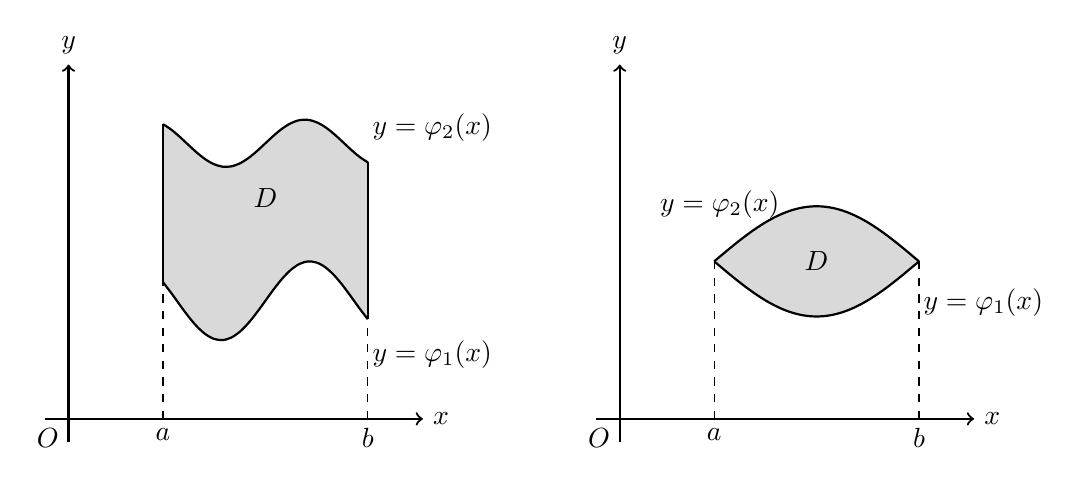
\begin{tikzpicture}
    \begin{scope}[shift={(0,0)},
        declare function={
            a = 1.2; b = 3.8;
            y1(\x) = 1.5 + 0.5*sin((\x-2.5)*160);
            y2(\x) = 3.5 + 0.3*sin((\x-2.5)*180);
        }]
        % 坐标轴
        \draw[->, thick] (-0.3,0) -- (4.5,0) node[right] {\(x\)};
        \draw[->, thick] (0,-0.3) -- (0,4.5) node[above] {\(y\)};
        \node[below left] at (0,0) {\(O\)};
    
        % 填充区域（包含左右竖直线段）
        \fill[gray!30]
            (a, {y1(a)}) --
            plot[domain=a:b, smooth] (\x, {y1(\x)}) --
            (b, {y2(b)}) --
            plot[domain=b:a, smooth] (\x, {y2(\x)}) --
            cycle;
    
        % 下边界曲线 + 右端点标签
        \draw[thick]
            plot[domain=a:b, smooth] (\x, {y1(\x)})
            node[below right, xshift=-2pt, yshift=-4pt] {\(y=\varphi_1(x)\)};
        % 上边界曲线 + 右端点标签
        \draw[thick]
            plot[domain=a:b, smooth] (\x, {y2(\x)})
            node[above right, xshift=-2pt, yshift=4pt] {\(y=\varphi_2(x)\)};
    
        % 左右竖直实线：连接上下端点
        \draw[thick] (a, {y1(a)}) -- (a, {y2(a)});
        \draw[thick] (b, {y1(b)}) -- (b, {y2(b)});
    
        % 虚线：x轴 → 上方曲线端点
        \draw[dashed] (a,0) -- (a, {y2(a)});
        \draw[dashed] (b,0) -- (b, {y2(b)});
        \node[below] at (a,0) {\(a\)};
        \node[below] at (b,0) {\(b\)};
    
        \node at (2.5, 2.8) {\(D\)};
    \end{scope}
    \begin{scope}[shift={(7,0)},
        declare function={
            a = 1.2; b = 3.8; k = 0.7;
            yLo(\x) = 2.0 - k*sin((\x-a)*180/(b-a));
            yHi(\x) = 2.0 + k*sin((\x-a)*180/(b-a));
        }]
        % 坐标轴
        \draw[->, thick] (-0.3,0) -- (4.5,0) node[right] {\(x\)};
        \draw[->, thick] (0,-0.3) -- (0,4.5) node[above] {\(y\)};
        \node[below left] at (0,0) {\(O\)};
    
        % 填充区域
        \fill[gray!30]
            (a, {yLo(a)}) --
            plot[domain=a:b, smooth] (\x, {yLo(\x)}) --
            (b, {yHi(b)}) --
            plot[domain=b:a, smooth] (\x, {yHi(\x)}) --
            cycle;
    
        % 下边界曲线 + 右端点标签
        \draw[thick]
            plot[domain=a:b, smooth] (\x, {yLo(\x)})
            node[below right, xshift=-2pt, yshift=-6pt] {\(y=\varphi_1(x)\)};
        % 上边界曲线 + 右端点标签
        \draw[thick]
            plot[domain=a:b, smooth] (\x, {yHi(\x)});
            
            \node[above, xshift=2pt, yshift=12pt] at (a, {yHi(a)}) {\(y=\varphi_2(x)\)};
    
        % 左右竖直实线：连接上下端点（此处上下端点重合，实线长度为零，可省略，但为保证一致性仍然画出）
        \draw[thick] (a, {yLo(a)}) -- (a, {yHi(a)});
        \draw[thick] (b, {yLo(b)}) -- (b, {yHi(b)});
    
        % 虚线：x轴 → 上方曲线端点
        \draw[dashed] (a,0) -- (a, {yHi(a)});
        \draw[dashed] (b,0) -- (b, {yHi(b)});
        \node[below] at (a,0) {\(a\)};
        \node[below] at (b,0) {\(b\)};
    
        \node at (2.5, 2) {\(D\)};
    \end{scope}
    \end{tikzpicture}
\end{center}

在区间 \([a,b]\) 上任意取定一点 \(x_0\)，作平行于 \(yOz\) 面的平面\(x=x_0\)，这平面截曲顶柱体所得的截面是一个以区间 \([\varphi_1(x_0),\varphi_2(x_0)]\) 为底、曲线\(z=f(x_0,y)\) 为曲边的曲边梯形，所以这截面的面积为$\int_{\varphi_1(x_0)}^{\varphi_2(x_0)} f(x_0,y)\,dy$，那么任意$x$处的截面面积就是$\int_{\varphi_1(x)}^{\varphi_2(x)} f(x,y)\,dy$，再对$x$积分，把面积累加起来，就得到曲顶柱体体积，也就是$\int_a^b\left[\int_{\varphi_1(x)}^{\varphi_2(x)} f(x,y)\,dy\right]dx$。

\begin{center}
    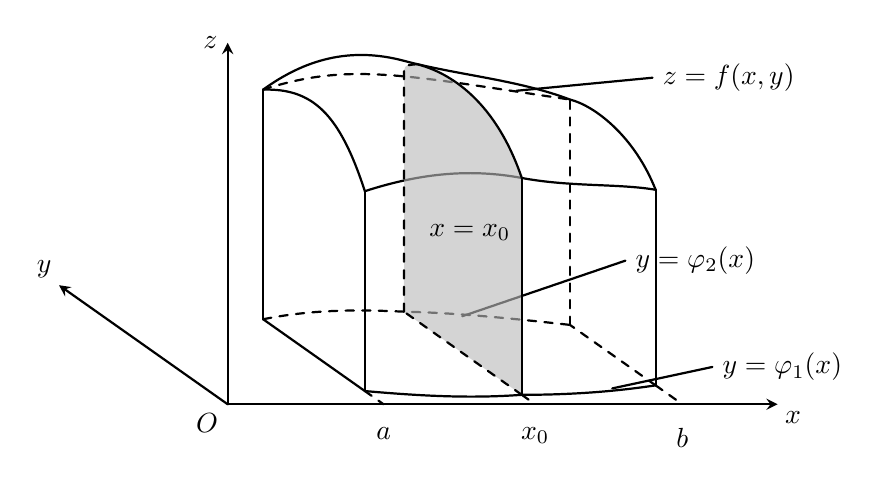
\begin{tikzpicture}[
      % 三维坐标在纸面上的斜投影方向
      x={(1.10cm,0cm)},
      y={(-0.68cm,0.48cm)},
      z={(0cm,1.08cm)},
      >=stealth,
      line cap=round,
      line join=round,
    ]
    
    % 关键点：下标 1、2 分别对应 y=phi_1(x)、y=phi_2(x)
    \coordinate (O)   at (0,0,0);
    \coordinate (A1)  at (1.80,0.35,0);
    \coordinate (A2)  at (1.80,2.25,0);
    \coordinate (M1)  at (3.55,0.25,0);
    \coordinate (M2)  at (3.55,2.45,0);
    \coordinate (B1)  at (5.25,0.50,0);
    \coordinate (B2)  at (5.25,2.10,0);
    
    % 上方曲面边界上的对应点
    \coordinate (A1t) at (1.80,0.35,2.35);
    \coordinate (A2t) at (1.80,2.25,2.70);
    \coordinate (M1t) at (3.55,0.25,2.55);
    \coordinate (M2t) at (3.55,2.45,2.95);
    \coordinate (B1t) at (5.25,0.50,2.30);
    \coordinate (B2t) at (5.25,2.10,2.65);
    
    % 坐标轴
    \draw[->,thick] (O) -- (6.35,0,0) node[below right=-1pt] {$x$};
    \draw[->,thick] (O) -- (0,3.15,0) node[above left=-1pt] {$y$};
    \draw[->,thick] (O) -- (0,0,4.25) node[left] {$z$};
    \node[below left] at (O) {$O$};
    
    % x 轴上的标记
    \node[below=5pt] at (1.80,0,0) {$a$};
    \node[below=5pt] at (3.55,0,0) {$x_0$};
    \node[below=5pt] at (5.25,0,0) {$b$};
    
    % 底面区域的边界
    \draw[thick]
      (A1) .. controls (2.45,0.20,0) and (2.95,0.16,0) .. (M1)
           .. controls (4.20,0.25,0) and (4.75,0.36,0) .. (B1);
    \draw[thick,dashed]
      (A2) .. controls (2.45,2.48,0) and (2.95,2.52,0) .. (M2)
           .. controls (4.15,2.42,0) and (4.72,2.26,0) .. (B2);
    \draw[thick] (A1) -- (A2);
    \draw[thick,dashed] (B1) -- (B2);
    
    % 背后的竖直母线
    \draw[thick] (A2) -- (A2t);
    \draw[thick,dashed] (B2) -- (B2t);
    
    
    
    
    % 两侧的竖直边界
    \draw[thick] (A1) -- (A1t);
    \draw[thick] (B1) -- (B1t);
    
    % 文字标注及引线
    \draw[thick]
      (4.15,1.32,3.10) -- (5.35,0.72,3.52)
      node[right] {$z=f(x,y)$};
    \draw[thick]
      (4.15,2.33,0) -- (5.55,1.55,1.00)
      node[right] {$y=\varphi_2(x)$};
    \draw[thick]
      (4.70,0.42,0) -- (5.72,0.20,0.35)
      node[right] {$y=\varphi_1(x)$};
    
    % 上方曲面的轮廓
    % 第一条光滑曲线 A1t → M1t → B1t
    \draw[thick]
      (A1t) .. controls (2.40,0.24,2.62) and (2.95,0.20,2.68) .. (M1t)
            .. controls (4.15,0.30,2.42) and (4.75,0.40,2.42) .. (B1t);
    
    \draw[thick,dashed]
      (A2t) .. controls (2.98,2.54,2.90) and (3.55,2.45,2.78) .. (B2t);
    
    % 第二条光滑曲线 A2t → M2t → B2t
    \draw[thick]
      (A2t) .. controls (2.42,2.48,2.95) and (2.98,2.54,3.08) .. (M2t)
            .. controls (4.12,2.36,2.82) and (4.73,2.25,2.82) .. (B2t);
    
    \draw[thick]
      (A1t) .. controls (1.80,0.82,3.05) and (1.80,1.32,3.13) .. (A2t);
    \draw[thick]
      (B1t) .. controls (5.25,0.90,2.76) and (5.25,1.65,2.78) .. (B2t);
    
    % x=x_0 处的截面 A(x_0)
    % 先填充，再描边；透明度可以改为 1 得到实心灰色
    \fill[gray!55,opacity=.62]
      (M1) -- (M2) -- (3.52,2.40,2.79) .. controls (3.53,2.42,2.91) .. (3.7,2.45,2.91) -- (3.7,2.45,2.91)
      .. controls (3.55,1.85,3.12) and (3.55,0.82,3.35) .. (M1t)
      -- cycle;
    \draw[thick,dashed] (M1) -- (M2);
    \draw[thick] (M1) -- (M1t);
    \draw[thick,dashed] (M2) -- (3.52,2.40,2.79);
    \draw[thick]
      (3.7,2.45,2.91) .. controls (3.55,1.85,3.12) and (3.55,0.82,3.35) .. (M1t);
    \draw[thick,dashed] (3.7,2.45,2.91) .. controls (3.53,2.42,2.91) .. (3.52,2.40,2.79);
    \node at (3.55,1.22,1.48) {$x=x_0$};
    
    
    \draw[thick,dashed] (1.80,0.35,0) -- (1.80,0,0);
    
    \draw[thick,dashed] (5.25,0.50,0) -- (5.25,0,0);
    
    \draw[thick,dashed] (3.55,0.25,0) -- (3.55,0,0);
    
    \end{tikzpicture}
\end{center}

如果区域 \(D\) 可以写成夹在两条水平线 \(y=c\) 与 \(y=d\) 之间，且左右两边分别是曲线 \(x=\psi_1(y)\) 和 \(x=\psi_2(y)\)的形式，即：
\[
D=\{(x,y)\mid c\le y\le d,\ \psi_1(y)\le x\le\psi_2(y)\}
\]

那么我们习惯上把这种区域称为 $Y$ 型区域。这时二重积分可以化成先对 \(x\) 后对 \(y\) 的二次积分：

\begin{theorem}{$Y$ 型区域的二重积分}{}
    若区域 \(D\) 是 $Y$ 型区域，则在区域 \(D\) 上的二重积分可化为：
\[
\iint_D f(x,y)\,dxdy = \int_c^d\left[ \int_{\psi_1(y)}^{\psi_2(y)} f(x,y)\,dx\right]dy = \int_c^d\ \int_{\psi_1(y)}^{\psi_2(y)} f(x,y)\,dxdy
\]
\end{theorem}

\begin{center}
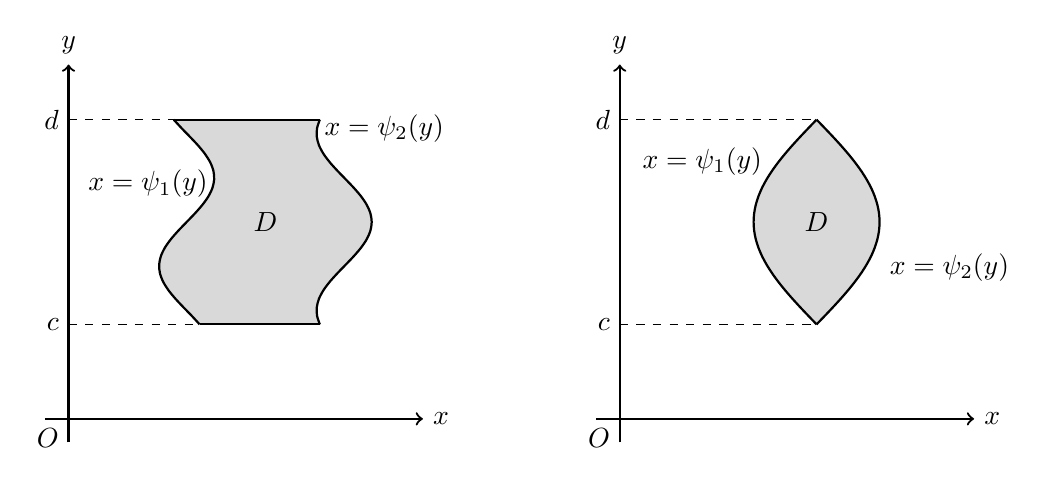
\begin{tikzpicture}
% ========= 左图：一般 y 型区域 =========
\begin{scope}[shift={(0,0)},
    declare function={
        c = 1.2; d = 3.8;
        psi1(\y) = 1.5 + 0.35*sin((\y-2.5)*160);
        psi2(\y) = 3.5 + 0.35*cos((\y-2.5)*160);
    }]
    % 坐标轴
    \draw[->, thick] (-0.3,0) -- (4.5,0) node[right] {\(x\)};
    \draw[->, thick] (0,-0.3) -- (0,4.5) node[above] {\(y\)};
    \node[below left] at (0,0) {\(O\)};

    % 填充区域
    \fill[gray!30]
        ({psi1(c)}, c) --
        plot[domain=c:d, smooth] ({psi1(\x)}, \x) --
        ({psi2(d)}, d) --
        plot[domain=d:c, smooth] ({psi2(\x)}, \x) --
        cycle;

    % 左边界曲线 + 标签（放在上端点）
    \draw[thick]
        plot[domain=c:d, smooth] ({psi1(\x)}, \x)
        node[above left, xshift=16pt, yshift=-32pt] {\(x=\psi_1(y)\)};
    % 右边界曲线 + 标签（放在上端点）
    \draw[thick]
        plot[domain=c:d, smooth] ({psi2(\x)}, \x)
        node[above right, xshift=-2pt, yshift=-12pt] {\(x=\psi_2(y)\)};

    % 上下水平实线（连接左右端点）
    \draw[thick] ({psi1(c)}, c) -- ({psi2(c)}, c);
    \draw[thick] ({psi1(d)}, d) -- ({psi2(d)}, d);

    % 虚线：从 y 轴到右曲线端点，标出 c 和 d
    \draw[dashed] (0,c) -- ({psi2(c)}, c);
    \draw[dashed] (0,d) -- ({psi2(d)}, d);
    \node[left] at (0,c) {\(c\)};
    \node[left] at (0,d) {\(d\)};

    % 区域标签
    \node at (2.5, 2.5) {\(D\)};
\end{scope}

% ========= 右图：上下端点重合的 y 型区域 =========
\begin{scope}[shift={(7,0)},
    declare function={
        c = 1.2; d = 3.8; k = 0.8;
        psiLo(\y) = 2.5 - k*sin((\y-c)*180/(d-c));
        psiHi(\y) = 2.5 + k*sin((\y-c)*180/(d-c));
    }]
    % 坐标轴
    \draw[->, thick] (-0.3,0) -- (4.5,0) node[right] {\(x\)};
    \draw[->, thick] (0,-0.3) -- (0,4.5) node[above] {\(y\)};
    \node[below left] at (0,0) {\(O\)};

    % 填充区域
    \fill[gray!30]
        ({psiLo(c)}, c) --
        plot[domain=c:d, smooth] ({psiLo(\x)}, \x) --
        ({psiHi(d)}, d) --
        plot[domain=d:c, smooth] ({psiHi(\x)}, \x) --
        cycle;

    % 左边界曲线 + 标签（放在上端点）
    \draw[thick]
        plot[domain=c:d, smooth] ({psiLo(\x)}, \x)
        node[above left, xshift=-16pt, yshift=-24pt] {\(x=\psi_1(y)\)};
    % 右边界曲线 + 标签（放在下端点，仿照 x 型对应图的标注方式）
    \draw[thick]
        plot[domain=c:d, smooth] ({psiHi(\x)}, \x);
    \node[above, xshift=48pt, yshift=12pt] at ({psiHi(c)}, c) {\(x=\psi_2(y)\)};

    % 上下水平实线：连接左右端点（此处端点重合，长度为零，可省略，保留以保持一致性）
    \draw[thick] ({psiLo(c)}, c) -- ({psiHi(c)}, c);
    \draw[thick] ({psiLo(d)}, d) -- ({psiHi(d)}, d);

    % 虚线：从 y 轴到重合点，标出 c 和 d
    \draw[dashed] (0,c) -- ({psiHi(c)}, c);
    \draw[dashed] (0,d) -- ({psiHi(d)}, d);
    \node[left] at (0,c) {\(c\)};
    \node[left] at (0,d) {\(d\)};

    % 区域标签
    \node at (2.5, 2.5) {\(D\)};
\end{scope}
\end{tikzpicture}
\end{center}

具体的操作和$X$ 型区域的二重积分类似，不再赘述。

先对哪个自变量积分，关键是积分区域。如果是$ X $型区域，就最后对$x$积分，先对$y$积分。如果是$ Y $型区域，就最后对$y$积分，先对$x$积分。也就是说，是什么区域就最后积哪个。

如果区域本身既不是$ X $型也不是$ Y $型，就用平行于坐标轴的直线把它切成几块，每块单独处理，再利用积分的区域可加性加起来就行了。

一般地，当我们写$\int_a^b\ \int_{\varphi_1(x)}^{\varphi_2(x)} f(x,y)\,dxdy$或者$\int_c^d\ \int_{\psi_1(y)}^{\psi_2(y)} f(x,y)\,dxdy$的时候，表示的其实是二重积分。形式上看着像是先对$\int_{\varphi_1(x)}^{\varphi_2(x)} f(x,y)\,dxdy$或者$\int_{\psi_1(y)}^{\psi_2(y)} f(x,y)\,dxdy$积分，再从$a$积到$b$或者从$c$积到$d$。然而这样其实是不合理的，因为第二个积分没有积分变量。

二重积分转换为两次定积分之后，就要处理这两个定积分的上下限。在实际应用中，我们通常用“画图穿线法”来确定它们的上下限。比如区域是$ X $型，就用一根平行于 \(y\) 轴的直线从下往上穿过区域，穿进去的边界就是下边界 \(y=\varphi_1(x)\)，穿出来的边界就是上边界 \(y=\varphi_2(x)\)，然后把这条线从左扫到右，就得到 \(x\) 的范围 \([a,b]\)。$Y $型区域也是类似的。

这么说肯定很难理解，我们看一个例子就明白了：

\begin{myexample}
    计算二重积分$\iint_D x \, d\sigma$，其中区域$D$是由$y$ 轴，直线$y=1$以及直线$x=y$围成的区域。

    我们首先要判断区域$D$是什么类型的区域。我们把直线$y=1$和直线$x=y$画出来，会发现它们与$y$ 轴围成了一个三角形。这个区域看成$X$ 型区域或者$Y$ 型区域都可以，这里作为示例，我们把它看成$Y$ 型区域计算。

    接下来就是“画图穿线法”的操作。判断区域为$Y$ 型，我们就要用一根平行于 \(x\) 轴的直线从左往右穿过这个区域，那么这根直线和区域$D$一定会有两个交点，我们分别记为$A$和$B$。然后比较大小，在左面的点小，作为积分下限，这里是\(x = 0\)。在右面的点大，作为积分上限，这里是\(x = y\)。

 \begin{center}
    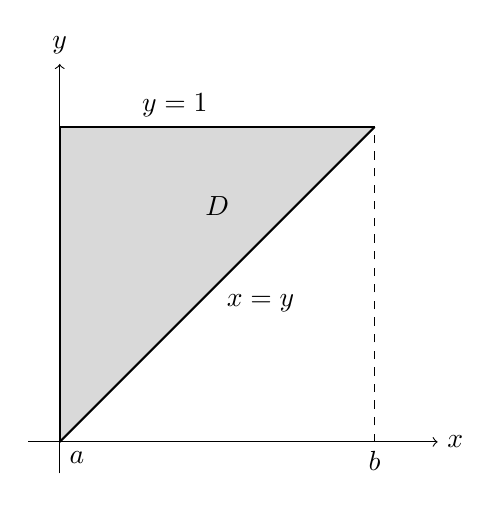
\begin{tikzpicture}[x=4cm, y=4cm]
        % 坐标轴
        \draw[->] (-0.1,0) -- (1.2,0) node[right] {$x$};
        \draw[->] (0,-0.1) -- (0,1.2) node[above] {$y$};
    
        % 填充区域 D: 0 <= x <= 1, x <= y <= 1
        \fill[gray!30] (0,0) 
            -- plot[domain=0:1, smooth] (\x, \x) 
            -- (1,1) 
            -- plot[domain=1:0, smooth] (\x, 1) 
            -- cycle;
    
        % 下边界曲线 y = x
        \draw[thick, domain=0:1, smooth] plot (\x, \x);
        \node[below right] at (0.5,0.5) {$x = y$};
        % 上边界直线 y = 1
        \draw[thick] (0,1) -- (1,1);
        \node[above left] at (0.5,1) {$y=1$};
        \draw[thick] (0,0) -- (0,1);
    
        % 右边界虚线及积分限 a, b
        \draw[dashed] (1,0) -- (1,1);
        \node[below] at (1,0) {$b$};
        \node[below right] at (0,0) {$a$};
    
        % 区域标签
        \node at (0.5,0.75) {$D$};
    \end{tikzpicture}
    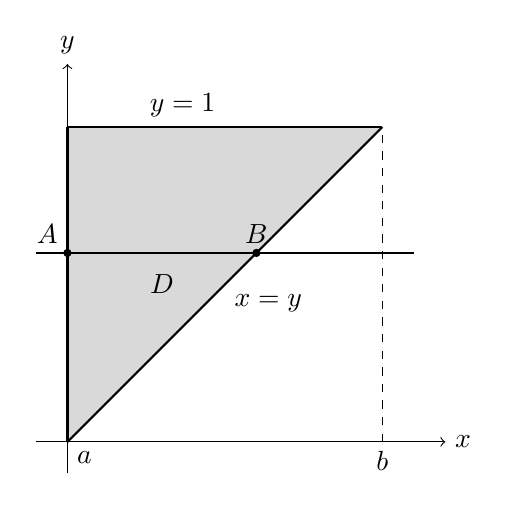
\begin{tikzpicture}[x=4cm, y=4cm]
        % 坐标轴
        \draw[->] (-0.1,0) -- (1.2,0) node[right] {$x$};
        \draw[->] (0,-0.1) -- (0,1.2) node[above] {$y$};
    
        % 填充区域 D: 0 <= x <= 1, x <= y <= 1
        \fill[gray!30] (0,0) 
            -- plot[domain=0:1, smooth] (\x, \x) 
            -- (1,1) 
            -- plot[domain=1:0, smooth] (\x, 1) 
            -- cycle;
    
        % 下边界曲线 y = x
        \draw[thick, domain=0:1, smooth] plot (\x, \x);
        \node[below right] at (0.5,0.5) {$x = y$};
        % 上边界直线 y = 1
        \draw[thick] (0,1) -- (1,1);
        \node[above left] at (0.5,1) {$y=1$};
        \draw[thick] (0,0) -- (0,1);
    
        % 右边界虚线及积分限 a, b
        \draw[dashed] (1,0) -- (1,1);
        \node[below] at (1,0) {$b$};
        \node[below right] at (0,0) {$a$};
        
    \draw[thick] (-0.1, 0.6) -- (1.1, 0.6);
    \node[above left] at (0,0.6) {$A$};
    \fill (0,0.6) circle (1.5pt);
    \node[above] at (0.6,0.6) {$B$};
    \fill (0.6,0.6) circle (1.5pt);
    
        % 区域标签
        \node at (0.3,0.5) {$D$};
    \end{tikzpicture}
\end{center}
   
那么我们就确定了上下限，得到第一重积分$\int_{0}^y x \, dx$，现在判断区间长度。这个区间从左扫到右，也就是$[0,1]$。由此我们就确定了区间，也得到了第二重积分$\int_0^1\ \int_{0}^y x \, dxdy$。那么我们现在就可以计算了。

先算第一重积分，这是一个对$x$积分的关于$y$的积分上限函数，积出来就是：

$$\int_{0}^y x \, dx=\left[\frac{1}{2}x^2\right]_0^y=\frac{1}{2}y^2$$

再代入第二重积分：

$$\int_0^1 \frac{1}{2}y^2 dy =\left[ \frac{1}{6}y^3\right]_0^1=\frac{1}{6}$$


所以二重积分$\iint_D x \, d\sigma=\frac{1}{6}$。
\end{myexample}


\begin{myexample}
    计算二重积分 $\iint_D (x+y) \, d\sigma$，其中区域$D$为抛物线\(y = x^2\) 和直线 \(y = x\) 围成的区域。

    我们首先先判断区域$D$是什么类型的区域。我们把抛物线\(y = x^2\) 和直线 \(y = x\) 画出来，就会发现它们围成的图形类似于一个弓形。这个区域看成$X$ 型区域或者$Y$ 型区域都可以，但是这里既然已经给出了\(y = x^2\) 和 \(y = x\)，为了方便，我们就把区域$D$看成$X$ 型区域。
    
    接下来就是“画图穿线法”的操作。判断区域为$X$ 型，我们就要用一根平行于 \(y\) 轴的直线从下往上穿过这个区域，那么这根直线和区域$D$一定会有两个交点，我们分别记为$A$和$B$。然后比较大小，在下面的点小，作为积分下限，这里是\(y = x^2\)。在上面的点大，作为积分上限，这里是\(y = x\)。

\begin{center}
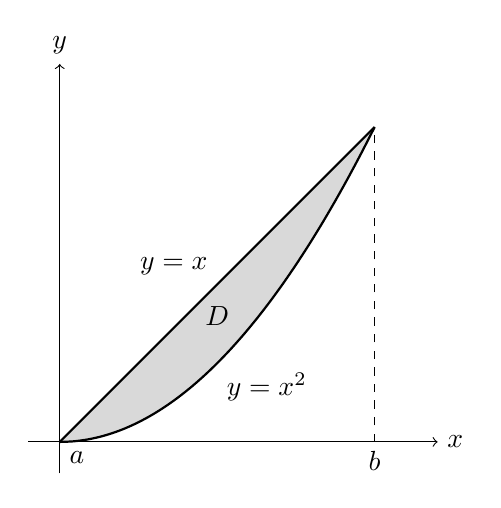
\begin{tikzpicture}[x=4cm, y=4cm]
    % 坐标轴
    \draw[->] (-0.1,0) -- (1.2,0) node[right] {$x$};
    \draw[->] (0,-0.1) -- (0,1.2) node[above] {$y$};

    % 填充 X 型区域 D: 0 <= x <= 1, x^2 <= y <= x
    \fill[gray!30] (0,0) 
        -- plot[domain=0:1, smooth] (\x, {\x*\x}) 
        -- (1,1) 
        -- plot[domain=1:0, smooth] (\x, {\x}) 
        -- cycle;

    % 下边界曲线 y = x^2
    \draw[thick, domain=0:1, smooth] plot (\x, {\x*\x});
        \node[below right] at (0.5,0.25) {$y=x^2$};
    % 上边界曲线 y = x
    \draw[thick, domain=0:1, smooth] plot (\x, {\x});
        \node[above left] at (0.5,0.5) {$y=x$};

    % 右边界虚线及 a, b 标注
    \draw[dashed] (1,0) -- (1,1);
    \node[below] at (1,0) {$b$};
    \node[below right] at (0,0) {$a$};

    % 区域标签
    \node at (0.5,0.4) {$D$};
\end{tikzpicture}
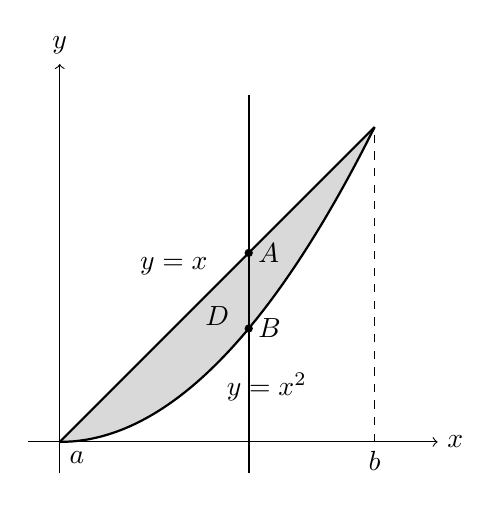
\begin{tikzpicture}[x=4cm, y=4cm]
    % 坐标轴
    \draw[->] (-0.1,0) -- (1.2,0) node[right] {$x$};
    \draw[->] (0,-0.1) -- (0,1.2) node[above] {$y$};

    % 填充 X 型区域 D: 0 <= x <= 1, x^2 <= y <= x
    \fill[gray!30] (0,0) 
        -- plot[domain=0:1, smooth] (\x, {\x*\x}) 
        -- (1,1) 
        -- plot[domain=1:0, smooth] (\x, {\x}) 
        -- cycle;

    % 下边界曲线 y = x^2
    \draw[thick, domain=0:1, smooth] plot (\x, {\x*\x});
        \node[below right] at (0.5,0.25) {$y=x^2$};
    % 上边界曲线 y = x
    \draw[thick, domain=0:1, smooth] plot (\x, {\x});
        \node[above left] at (0.5,0.5) {$y=x$};

    % 右边界虚线及 a, b 标注
    \draw[dashed] (1,0) -- (1,1);
    \node[below] at (1,0) {$b$};
    \node[below right] at (0,0) {$a$};
    
    \draw[thick] (0.6, -0.1) -- (0.6, 1.1);
    \node[right] at (0.6, 0.6) {$A$};
    \fill (0.6,0.6) circle (1.5pt);
    \node[right] at (0.6, 0.36) {$B$};
    \fill (0.6, 0.36) circle (1.5pt);

    % 区域标签
    \node at (0.5,0.4) {$D$};
\end{tikzpicture}
\end{center}

那么我们就确定了上下限，得到第一重积分$\int_{x^2}^x (x+y) \, dy$，现在判断区间长度。这个区间从左扫到右，其实就是\(y = x^2\) 和 \(y = x\)的交点，也就是$[0,1]$。由此我们就确定了区间，也得到了第二重积分$\int_0^1\ \int_{x^2}^x (x+y) \, dydx$。那么我们现在就可以计算了。

第一重积分其实是一个关于$x$的积分上限函数，但是这里是对$y$积分，我们先把它积出来，也就是：

$$\int_{x^2}^x (x+y) \, dy
= \left[ xy + \frac{y^2}{2} \right]_{x^2}^{x} = \frac{3}{2}x^2 - x^3 - \frac{1}{2}x^4$$

再代入到第二重积分里，就是：

$$\int_0^1 (\frac{3}{2}x^2 - x^3 - \frac{1}{2}x^4) dx=\left[ \frac{1}{2}x^3 - \frac{1}{4}x^4 - \frac{1}{10}x^5 \right]_0^1=\frac{3}{20}$$

所以二重积分$\iint_D (x+y) \, d\sigma=\frac{3}{20}$。
\end{myexample}

\begin{myexample}
    计算二重积分$\iint_D (x+y) \, d\sigma$，其中区域$D$ 是由曲线 $y = \sin x$、$y = \cos x$、$x = 0$ 和 $x = \dfrac{\pi}{2}$ 围成的闭区域。

    我们首先判断区域 $D$ 是什么类型的区域。把曲线 $y = \sin x$、$y = \cos x$ 与直线 $x = 0$、$x = \dfrac{\pi}{2}$ 画出来，就会发现它们围成了两个曲边三角形。这个区域其实是 $X$ 型区域，但是在区间 $[0,\frac{\pi}{2}]$ 上，两条曲线相交于 $x = \frac{\pi}{4}$，将区域分成了左右两部分。

    接下来就是“画图穿线法”的操作。判断区域为 $X$ 型，我们用一根平行于 $y$ 轴的直线从下往上穿过这个区域，直线与区域 $D$ 会有两个交点。但是区域分左右两部分，我们就要分别讨论。

    我们记区间 $[0,\frac{\pi}{4}]$ 上的区域为$D_1$。在该区间上，曲线 $y = \cos x$ 在 $y = \sin x$ 的上方，因此直线先交 $y = \sin x$，再交 $y = \cos x$。所以这部分的积分下限为 $y = \sin x$，积分上限为 $y = \cos x$。

    我们记区间 $[\frac{\pi}{4},\frac{\pi}{2}]$ 上的区域为$D_2$。在该区间上，曲线 $y = \sin x$ 在 $y = \cos x$ 的上方，因此直线先交 $y = \cos x$，再交$y = \sin x$。所以这部分的积分下限为 $y = \cos x$，积分上限为 $y = \sin x$。

\begin{center}
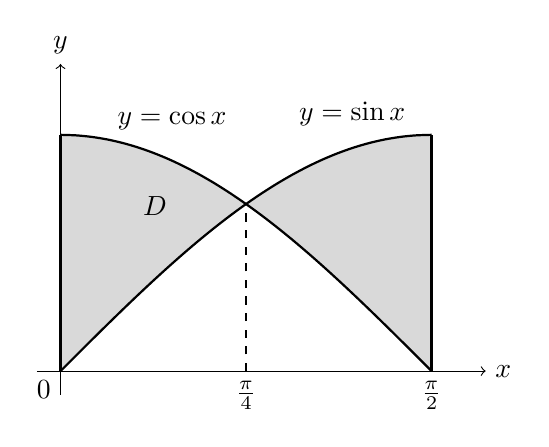
\begin{tikzpicture}[x=3cm, y=3cm, scale=1]
    % 坐标轴
    \draw[->] (-0.1,0) -- (1.8,0) node[right] {$x$};
    \draw[->] (0,-0.1) -- (0,1.3) node[above] {$y$};

    % 左半区域填充 (0≤x≤π/4, sin x ≤ y ≤ cos x)
    \fill[gray!30] (0,0) -- plot[domain=0:pi/4, smooth] (\x, {sin(\x r)}) --
        (pi/4, {cos(pi/4 r)}) -- plot[domain=pi/4:0, smooth] (\x, {cos(\x r)}) -- cycle;
    % 右半区域填充 (π/4≤x≤π/2, cos x ≤ y ≤ sin x)
    \fill[gray!30] (pi/4, {cos(pi/4 r)}) -- plot[domain=pi/4:pi/2, smooth] (\x, {cos(\x r)}) --
        (pi/2,1) -- plot[domain=pi/2:pi/4, smooth] (\x, {sin(\x r)}) -- cycle;

        \draw[thick] (pi/2,0) -- (pi/2,1);
        \draw[thick] (0,0) -- (0,1);

    % 曲线
    \draw[thick, domain=0:pi/2, smooth] plot (\x, {sin(\x r)});
    \node[above left] at (1.5, {sin(1.5 r)}) {$y=\sin x$};
    \draw[thick, domain=0:pi/2, smooth] plot (\x, {cos(\x r)});
    \node[above right] at (0.2, {cos(0.2 r)}) {$y=\cos x$};

    % 交点虚线
    \draw[dashed] (pi/4,0) -- (pi/4, {sin(pi/4 r)});
    \node[below] at (pi/4,0) {$\frac{\pi}{4}$};

    % 边界标注
    \node[below left] at (0,0) {$0$};
    \node[below] at (pi/2,0) {$\frac{\pi}{2}$};

    % 区域标签
    \node at (0.4,0.7) {$D$};
\end{tikzpicture}
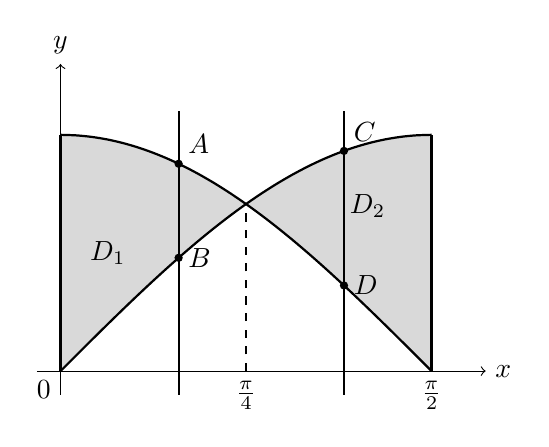
\begin{tikzpicture}[x=3cm, y=3cm, scale=1]
    % 坐标轴
    \draw[->] (-0.1,0) -- (1.8,0) node[right] {$x$};
    \draw[->] (0,-0.1) -- (0,1.3) node[above] {$y$};

    % 填充区域（简化填充）
    \fill[gray!30] (0,0) -- plot[domain=0:pi/4, smooth] (\x, {sin(\x r)}) --
        (pi/4, {cos(pi/4 r)}) -- plot[domain=pi/4:0, smooth] (\x, {cos(\x r)}) -- cycle;
    \fill[gray!30] (pi/4, {cos(pi/4 r)}) -- plot[domain=pi/4:pi/2, smooth] (\x, {cos(\x r)}) --
        (pi/2,1) -- plot[domain=pi/2:pi/4, smooth] (\x, {sin(\x r)}) -- cycle;
        \draw[thick] (pi/2,0) -- (pi/2,1);
        \draw[thick] (0,0) -- (0,1);

    % 曲线
    \draw[thick, domain=0:pi/2, smooth] plot (\x, {sin(\x r)});
    \draw[thick, domain=0:pi/2, smooth] plot (\x, {cos(\x r)});

    \draw[dashed] (pi/4,0) -- (pi/4, {sin(pi/4 r)});
    \node[below] at (pi/4,0) {$\frac{\pi}{4}$};

    % 边界标注
    \node[below left] at (0,0) {$0$};
    \node[below] at (pi/2,0) {$\frac{\pi}{2}$};

    % 穿线法：左段 x=0.5
    \draw[thick] (0.5, -0.1) -- (0.5, 1.1);
    \fill (0.5, {cos(0.5 r)}) circle (1.5pt) node[above right] {$A$};
    \fill (0.5, {sin(0.5 r)}) circle (1.5pt) node[right] {$B$};

    % 穿线法：右段 x=1.2
    \draw[thick] (1.2, -0.1) -- (1.2, 1.1);
    \fill (1.2, {sin(1.2 r)}) circle (1.5pt) node[above right] {$C$};
    \fill (1.2, {cos(1.2 r)}) circle (1.5pt) node[right] {$D$};

    \node at (0.2,0.5) {$D_1$};
    \node at (1.3,0.7) {$D_2$};
\end{tikzpicture}
\end{center}

    那么原积分就可以写成两部分之和。我们记区域$D_1$上的二重积分为$I_1$，记区域$D_2$上的二重积分为$I_2$，则$\iint_D (x+y) \, d\sigma=I_1+I_2$。

    先算$I_1$，我们刚刚确定了$I_1$的第一重积分的积分下限为 $y = \sin x$，积分上限为 $y = \cos x$，积出来就是：
    \[
    \int_{\sin x}^{\cos x} (x+y) \, dy=\left[ xy + \frac{y^2}{2} \right]_{\sin x}^{\cos x} = x\cos x - x\sin x + \frac{\cos 2x}{2}
    \]

    $I_1$的区间是$[0,\frac{\pi}{4}]$，所以第二重积分就是：
    \[
    \int_0^{\frac{\pi}{4}} (x\cos x - x\sin x + \frac{\cos 2x}{2}) \, dx=[x\sin x + \cos x + x\cos x - \sin x + \frac{1}{4}\sin 2x]_0^{\frac{\pi}{4}}=\frac{\pi\sqrt{2}-3}{4}
    \]

    同理可计算$I_2$。$I_2$的第一重积分的积分下限为$y = \cos x$，积分上限为 $y = \sin x$，所以：
    \[
    \int_{\cos x}^{\sin x} (x+y) \, dy=\left[ xy + \frac{y^2}{2} \right]_{\cos x}^{\sin x}=x\sin x - x\cos x - \frac{\cos 2x}{2}
    \]

    $I_2$的区间是$[\frac{\pi}{4},\frac{\pi}{2}]$，所以：
    \[
    \int_{\frac{\pi}{4}}^{\frac{\pi}{2}} (x\sin x - x\cos x - \frac{\cos 2x}{2}) \, dx=[-x\cos x + \sin x - x\sin x - \cos x - \frac{1}{4}\sin 2x]_{\frac{\pi}{4}}^{\frac{\pi}{2}}=\frac{5+\pi\sqrt{2}-2\pi}{4}
    \]

    最后相加得：
    \[\iint_D (x+y) \, d\sigma = I_1 + I_2 = \frac{\pi(\sqrt{2}-1)+1}{2}\]
\end{myexample}

有时我们会遇到一个写好了的累次积分，但按原顺序很难积或者积不出来。这时候我们可以根据上下限画出积分区域，然后交换积分次序，往往就能化难为易。

所谓交换积分次序，其实就是把$X$ 型区域看成$Y$ 型区域再去算，把$Y$ 型区域看成$X$ 型区域再去算。

\begin{myexample}
交换累次积分 \(\int_0^2\left[\int_{y^2}^{4} f(x,y)\,dx\right]dy\) 的积分次序。

观察原积分，我们发现这是一个先对$x$积分，再对$y$积分的二重积分，那么也就是说区域 \(D\) 是个$Y$ 型区域。根据原积分上下限，区域 \(D\) 可以表示为：
\[
D=\{(x,y)\mid 0\le y\le 2,\ y^2\le x\le 4\}
\]

我们把它画出来，就是：
\begin{center}
    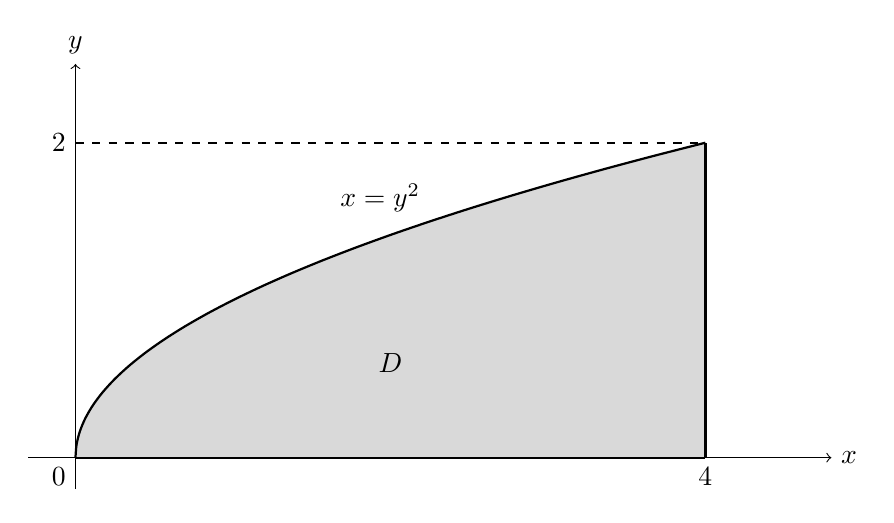
\begin{tikzpicture}[x=2cm, y=2cm]
        % 坐标轴
        \draw[->] (-0.3,0) -- (4.8,0) node[right] {$x$};
        \draw[->] (0,-0.2) -- (0,2.5) node[above] {$y$};
    
        % 填充积分区域 D: 0<=y<=2, y^2<=x<=4
        \fill[gray!30] (0,0) 
            -- (4,0) 
            -- (4,2) 
            -- plot[domain=2:0, smooth] ({\x*\x}, \x) 
            -- cycle;
    
        % 左边界曲线 x = y^2  (即 y = sqrt{x})
        \draw[thick, domain=0:2, smooth] plot ({\x*\x}, \x);
        \node[above left] at (2.25,1.5) {$x=y^2$};
    
        % 右边界直线 x = 4
        \draw[thick] (4,0) -- (4,2);
        \draw[thick,dashed] (0,2) -- (4,2);
        \draw[thick] (0,0) -- (4,0);
    
        % 坐标刻度
        \node[below] at (4,0) {$4$};
        \node[left] at (0,2) {$2$};
        \node[below left] at (0,0) {$0$};
    
        % 区域标签
        \node at (2,0.6) {$D$};
    \end{tikzpicture}
\end{center}

因此把区域 \(D\) 转写成$X$型，得：
\[
D=\{(x,y)\mid 0\le x\le 4,\ 0\le y\le\sqrt{x}\}
\]

交换次序后得到：
\[
\int_0^2\left[\int_{y^2}^{4} f(x,y)\,dx\right]dy = \int_0^4\left[\int_0^{\sqrt{x}} f(x,y)\,dy\right]dx
\]

\end{myexample}


\begin{myexample}
求$\int_{0}^{1} \left[ \int_{x}^{1} e^{y^{2}} \, dy \right] dx$。

我们发现，这个累次积分其中的$e^{y^{2}}$是一个典型的“积不出”积分，也就是说如果直接求，我们根本没办法求出它的值。那么这个时候我们就要考虑一下交换积分次序了。

原积分是先对$y$积分，再对$x$积分，也就是说这个区域是个$X$型区域。我们把这个区域画出来：
    
\begin{center}
        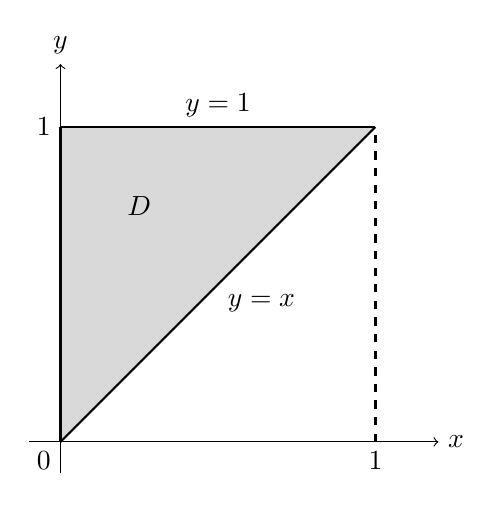
\begin{tikzpicture}[x=4cm, y=4cm]
        % 坐标轴
        \draw[->] (-0.1,0) -- (1.2,0) node[right] {$x$};
        \draw[->] (0,-0.1) -- (0,1.2) node[above] {$y$};
    
        % 填充区域 D: 0<=x<=1, x<=y<=1
        \fill[gray!30] (0,0) -- (0,1) -- (1,1) -- cycle;
    
        % 下边界 y = x
        \draw[thick, domain=0:1, smooth] plot (\x, \x);
        \node[below right] at (0.5,0.5) {$y=x$};
    
        % 上边界 y = 1
        \draw[thick] (0,1) -- (1,1);
        \node[above] at (0.5,1) {$y=1$};
    
        % 左边界 x=0 (与y轴重合)
        \draw[thick] (0,0) -- (0,1);
    
        \draw[thick,dashed] (1,0) -- (1,1);
    
        % 坐标标注
        \node[below] at (1,0) {$1$};
        \node[left] at (0,1) {$1$};
        \node[below left] at (0,0) {$0$};
    
        % 区域标签
        \node at (0.25,0.75) {$D$};
    \end{tikzpicture}
\end{center}

再把它转写成$Y$型区域，就得到：
\[
\int_{0}^{1} \left[ \int_{0}^{y} e^{y^{2}} \, dx \right] dy
\]

这里要注意，括号里的积分是对$x$的积分，也就是说和$y$完全无关，因此我们可以直接把$e^{y^{2}}$提出来，这个积分就变成：
\[
\int_{0}^{1} e^{y^{2}} \left[ \int_{0}^{y} \, dx \right] dy
\]

那么原积分就是：
\[
\int_{0}^{1} \left[ \int_{x}^{1} e^{y^{2}} \, dy \right] dx=\int_{0}^{1} e^{y^{2}} \left[ \int_{0}^{y} \, dx \right] dy=\int_{0}^{1} y \, e^{y^{2}} \, dy=\left[\frac{1}{2}e^{y^2}\right]_{0}^{1}=\frac{1}{2} (e - 1)
\]
\end{myexample}

总结一下，要求二重积分，首先要确定积分区域的类型。然后用“画图穿线法”确定第一重积分的上下限，如果是$X$型区域就从下往上穿，$Y$型区域就从左往右穿，也就是从小往大穿，小的作为积分下限，大的作为积分上限。把第一重积分积出来之后，再根据区间，确定第二重积分的上下限，把第一重积分积出来的结果代入第二重积分，就能求出值了。


\subsection{二重积分的极坐标形式}
有些二重积分的积分区域的边界是圆弧或射线，或者被积函数里出现了 \(x^2+y^2\) 类似的项。这时要是还用直角坐标去算，不仅上下限很难写，积分本身也可能变得十分复杂。这时，就可以考虑利用极坐标来计算二重积分。

我们假定读者已经对极坐标有基本的了解，所以我们直接进入极坐标形式下二重积分的计算。与直角坐标不同的是，在极坐标下，面积微元$d\sigma$不再是简单的$dxdy$，而是变成另一种形式。


\begin{center}
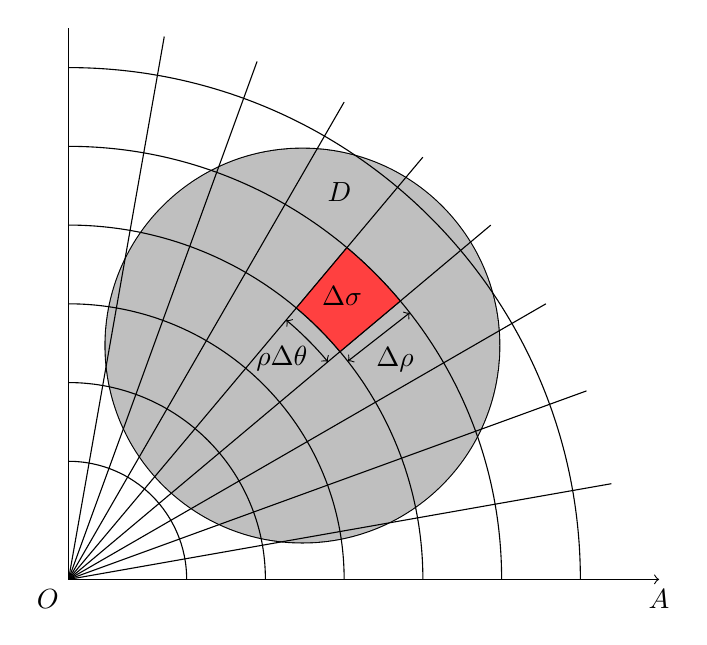
\begin{tikzpicture}

% 4. 绘制图形区域 D (粗线圆)
    \draw[thick] (45:4.2) circle (2.5);
    \fill[gray!50] (45:4.2) circle (2.5);

    % 1. 定义原点和极轴
    \coordinate (O) at (0,0);
    \coordinate (A) at (7.5,0);
    
    % 2. 绘制极网格 (灰度射线和圆弧)
    \foreach \angle in {10,20,30,40,50,60,70,80,90} {
        \draw (O) -- (\angle:7);
    }
    % 圆弧: 半径从 1.5 到 7.5，步长 1
    \foreach \r in {1.5,2.5,3.5,4.5,5.5,6.5} {
        \draw (0:\r) arc (0:90:\r);
    }

    % 3. 绘制极轴 OA (粗线，带箭头)
    \draw[->] (O) -- (A) node[below] {\(A\)};
    \node[below left] at (O) {\(O\)};

    

    

    % 5. 绘制阴影微元 \Delta\sigma_i (填充并描边)
    \fill[red!75] (40:4.5) arc (40:50:4.5) -- (50:5.5) arc (50:40:5.5) -- cycle;
    \draw (40:4.5) arc (40:50:4.5) -- (50:5.5) arc (50:40:5.5) -- cycle;

    % 6. 添加标注和向量
    % 标注 D
    \node at (55:6) {\(D\)};
    
    % 标注微元 \Delta\sigma_i
    \node at (46:5) {\(\Delta\sigma\)};

    % 标注 \Delta\theta_i (使用带箭头的弧线)
    \draw[<->, thin] (40:4.3) arc (40:50:4.3);
    \node at (46:3.9) {\(\rho\Delta\theta\)};

    % 标注 \Delta \r (使用带箭头的直线)
    \draw[<->, thin] (38:4.5) -- (38:5.5);
    \node at (34:5.0) {\(\Delta\rho\)};


\end{tikzpicture}
\end{center}

我们知道，在极坐标下，确定一个点需要确定极径$\rho$和极角$\theta$。与直角坐标类似，我们取一个极小的$\Delta\rho$和$\Delta \theta$，那么极径从$\rho$变化到$\rho+\Delta\rho$，极角从$\theta$变化到$\theta+\Delta \theta$，这时候的面积微元就是一个“曲边矩形”，矩形的边长就是$\Delta\rho$，弧长就是$\rho\Delta \theta$和$(\rho+\Delta\rho)\cdot \Delta \theta$。当$\Delta \theta$和$\Delta\rho$足够小的时候，我们就可以认为$\rho\Delta \theta$与$(\rho+\Delta\rho)\cdot \Delta \theta$相等，“曲边矩形”可以近似为矩形，面积也可以认为是$\Delta\rho \cdot \rho\Delta \theta$。然后我们取微分，那么面积就是$d\rho \cdot \rho d\theta$，也就是$\rho d\rho d\theta$。这就是极坐标下的面积微元。

如果区域 \(D\) 可以写成夹在两条射线 \(\theta=\alpha\) 与 \(\theta=\beta\) 之间，且内外边界分别是曲线 \(\rho=\rho_1(\theta)\) 和 \(\rho=\rho_2(\theta)\) 的形式，即：
\[
D=\{(\rho,\theta)\mid \alpha\le\theta\le\beta,\ \rho_1(\theta)\le \rho\le \rho_2(\theta)\}
\]

那么我们习惯上把这种区域称为极坐标下的标准区域。这时二重积分就可以化成先对 \(\rho\) 后对 \(\theta\) 的二次积分：

\begin{theorem}{极坐标下的二重积分}{}
    若区域 \(D\) 在极坐标下可表示为 \(\alpha\le\theta\le\beta,\ \rho_1(\theta)\le \rho\le \rho_2(\theta)\)，则
    \[
    \iint_D f(\rho,\theta)\,d\sigma = \iint_D f(\rho,\theta)\,\rho d\rho d\theta = \int_\alpha^\beta\left[\int_{\rho_1(\theta)}^{\rho_2(\theta)} f(\rho,\theta)\,\rho\,d\rho\right]d\theta
    \]
\end{theorem}

其中$\rho\ge 0$，$0\le \theta \le2\pi$。一般我们先积$\rho$，再积$\theta$。注意极坐标下的面积微元是$\textcolor{red}{\rho}d\rho d\theta$，不是$d\rho d\theta$。

有时候，我们想把直角坐标的二重积分转换为极坐标来算，那么这要怎么操作呢？我们只需要令$x=\rho\cos\theta$，$y=\rho\sin\theta$，再用极坐标计算就可以了。

\begin{theorem}{二重积分变换公式}{}
    \[
    \iint_D f(x,y)\,d\sigma = \iint_D f(x,y)\,dxdy = \iint_D f(\rho\cos\theta,\rho\sin\theta)\,\rho d\rho d\theta
    \]
\end{theorem}

计算极坐标下的二重积分的操作思路和直角坐标时如出一辙。我们先把 \(\theta\) 固定住，那么从极点出发、极角为 \(\theta\) 的射线穿进区域 \(D\) 时碰到的第一条边界就是 \(\rho=\rho_1(\theta)\)，穿出区域时碰到的边界就是 \(\rho=\rho_2(\theta)\)。于是沿着这条射线把函数值从 \(\rho_1(\theta)\) 到 \(\rho_2(\theta)\) 积起来，就得到了对应于这个 \(\theta\) 的一片“累积量”，然后再让 \(\theta\) 从 \(\alpha\) 扫到 \(\beta\)，把所有这样的片累加起来，就得到了整个二重积分。这和直角坐标下“先积一条线，再扫一个面”的做法完全是一样的，只不过是把直线换成了射线。

那么，怎么确定上下限呢？我们依旧用“画图穿线法”，只是在极坐标下，穿区域的线变成了从极点出发的射线。让射线绕着极点，从角度 \(\alpha\) 开始，沿逆时针方向扫到 \(\beta\)。在每一个角度上，射线进入区域的那一点就是积分下限 \(\rho=\rho_1(\theta)\)，穿出区域的那一点就是积分上限 \(\rho=\rho_2(\theta)\)。扫过的角度范围就是 \(\theta\) 的积分区间。也正因如此，所以极坐标下的二重积分基本都是先对$\rho$积分再对$\theta$积分。

和直角坐标一样，我们来看几个例子：

\begin{myexample}
    计算二重积分 \(\iint_D (x^2+y^2)\,d\sigma\)，其中区域 \(D\) 是由圆 \(x^2+y^2=1\) 围成的闭区域。

    我们将原积分化为极坐标形式。令$x = \rho\cos\theta$，$y = \rho\sin\theta$，则$d\sigma = \rho\,d\rho\,d\theta$，原积分化为$\iint_D \rho^2 \cdot \rho\,d\rho\,d\theta$。区域 \(D\) 化为$\rho^2\le1$。

    我们画出区域 \(D\)，再用“画图穿线法”确定上下限。先从极点引出一条射线，这条射线在从极点 \(\rho=0\) 出发，穿出圆时到达 \(\rho=1\)，所以积分下限是 \(\rho=0\)，积分上限是 \(\rho=1\)。让它逆时针扫过 \(0\) 到 \(2\pi\)，积分区间就是$[0,2\pi]$。

    \begin{center}
    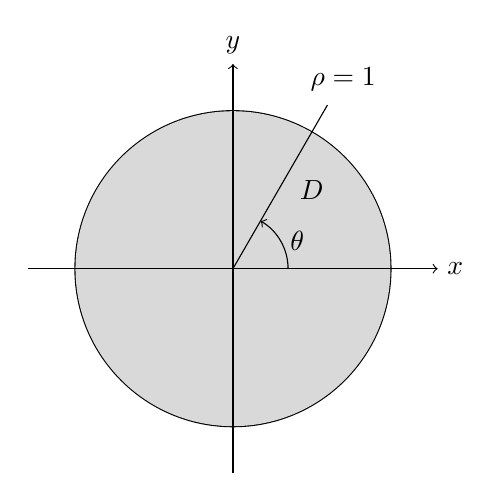
\begin{tikzpicture}[scale=2]
        % 单位圆
        \draw[thick] (0,0) circle (1);
        \fill[gray!30] (0,0) circle (1);

        % 极轴
        \draw[->] (-1.3,0) -- (1.3,0) node[right] {$x$};
        \draw[->] (0,-1.3) -- (0,1.3) node[above] {$y$};

        % 射线示例
        \draw[] (0,0) -- (60:1.2);
        \draw[->] (0.35,0) arc (0:60:0.35) node[midway, right] {$\theta$};

        \node at (0.5,0.5) {$D$};
        \node at (0.7,1.2) {$\rho=1$};

    \end{tikzpicture}
    \end{center}

    于是原积分化为：
    \[
\iint_D \rho^2 \cdot \rho\,d\rho\,d\theta = \int_{0}^{2\pi} \int_{0}^{1} \rho^3\,d\rho\,d\theta
    \]

    先算第一重积分：
    \[
    \int_{0}^{1} \rho^3\,d\rho = \left[ \frac{\rho^4}{4} \right]_{0}^{1} = \frac{1}{4}
    \]

    再代入第二重积分：
    \[
    \int_{0}^{2\pi} \frac{1}{4}\,d\theta = \frac{1}{4} \cdot 2\pi = \frac{\pi}{2}
    \]

    所以二重积分 \(\iint_D (x^2+y^2)\,d\sigma=\frac{\pi}{2}\)。
\end{myexample}

\begin{myexample}
    计算二重积分 \(\iint_D \sqrt{x^2+y^2}\,d\sigma\)，其中区域 \(D\) 是由心脏线 \(\rho=1+\cos\theta\) 围成的闭区域。

    同理，我们令$x = \rho\cos\theta$，$y = \rho\sin\theta$，则$d\sigma = \rho\,d\rho\,d\theta$，原积分化为$\iint_D \rho \cdot \rho\,d\rho\,d\theta$，区域 \(D\) 的边界由极坐标方程直接给出了。

    我们先画出区域 \(D\)，再用“画图穿线法”确定上下限。对于每一个角度 \(\theta\)，射线从极点出发，穿进区域时 \(\rho=0\)，穿出时上边界 \(\rho=1+\cos\theta\)。因此积分下限就是\(\rho=0\)，积分上限就是\(\rho=1+\cos\theta\)。\(\theta\)从\(0\) 到 \(2\pi\)能画出整个边界，所以积分区间就是$[0,2\pi]$。

    \begin{center}
    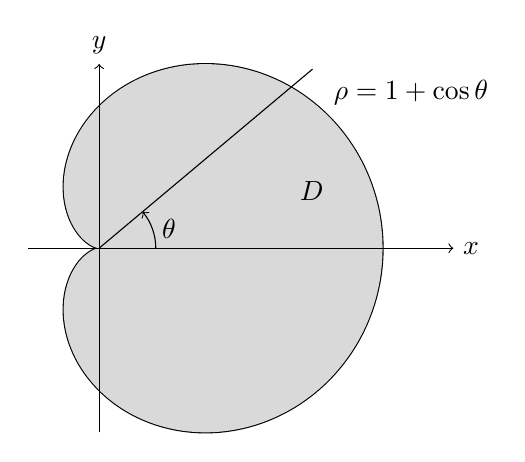
\begin{tikzpicture}[scale=1.8]

        % 心脏线
        \draw[thick, domain=0:360, smooth,samples=200] plot (\x:{1+cos(\x)});
        \fill[gray!30] plot[domain=0:360, smooth,samples=200] (\x:{1+cos(\x)}) -- cycle;

        \draw[->] (-0.5,0) -- (2.5,0) node[right] {$x$};
        \draw[->] (0,-1.3) -- (0,1.3) node[above] {$y$};

        % 射线示例
        \draw (0,0) -- (40:{1.2+cos(40)});
        \draw[->] (0.4,0) arc (0:40:0.4) node[midway, right] {$\theta$};

        \node at (1.5,0.4) {$D$};
        \node at (2.2,1.1) {$\rho=1+\cos\theta$};
    \end{tikzpicture}
    \end{center}

    于是原积分化为：
    \[
    \iint_D \rho\,d\sigma = \int_0^{2\pi}\left[\int_0^{1+\cos\theta} \rho\cdot \rho\,d\rho\right]d\theta
    = \int_0^{2\pi}\left[\int_0^{1+\cos\theta} \rho^2\,d\rho\right]d\theta
    \]

    先算第一重积分：
    \[
    \int_0^{1+\cos\theta} \rho^2\,d\rho = \left[\frac{\rho^3}{3}\right]_0^{1+\cos\theta} = \frac{(1+\cos\theta)^3}{3}
    \]

    再代入第二重积分：
    \[
    \frac13\int_0^{2\pi} (1+\cos\theta)^3\,d\theta = \frac13\left[\int_0^{2\pi}1\,d\theta + 3\int_0^{2\pi}\cos^2\theta\,d\theta\right]
    = \frac13(2\pi + 3\pi) = \frac{5\pi}{3}
    \]

    所以二重积分 \(\iint_D \sqrt{x^2+y^2}\,d\sigma = \frac{5\pi}{3}\)。
\end{myexample}

\begin{myexample}
    计算二重积分 \(\iint_D \arctan\frac{y}{x}\,d\sigma\)，其中区域 \(D\) 是由圆 \(x^2+y^2=1\)，\(x^2+y^2=4\) 与射线 \(y=x\ (x\ge 0)\)，\(y=0\ (x\ge 0)\) 所围成的在第一象限的部分。

    令$x = \rho\cos\theta$，$y = \rho\sin\theta$，先化简被积函数：
    \[
    \arctan\frac{y}{x}=\arctan\frac{\rho\sin\theta}{\rho\cos\theta}=\arctan\tan\theta=\theta
    \]

    所以原积分就是 \(\iint_D \theta\,d\sigma\)，区域 \(D\)是夹在两个圆和两条射线之间的环形扇区。从极点出发的射线，在角度 \(\theta\) 从 \(0\) 扫到 \(\frac{\pi}{4}\) 的过程中，先穿入小圆边界 \(\rho=1\)，再穿出大圆边界 \(\rho=2\)。所以积分下限是\(\rho=1\)，积分上限是\(\rho=2\)，积分区间是\([0,\frac{\pi}{4}]\)。

\begin{center}
    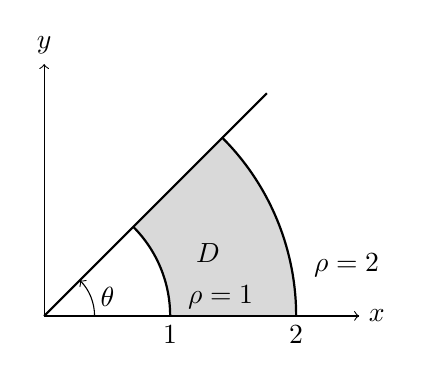
\begin{tikzpicture}[scale=1.6]

        % 填充区域（仍保持在 0°~45°，r=1~2）
        \fill[gray!30] 
            (0:1) arc (0:45:1) -- 
            (45:2) arc (45:0:2) -- cycle;

        % 坐标轴（仅正半轴）
        \draw[->] (0,0) -- (2.5,0) node[right] {$x$};
        \draw[->] (0,0) -- (0,2) node[above] {$y$};

        % 射线
        \draw[dashed] (0,0) -- (45:2.5);
        \draw[thick] (0,0) -- (2.5,0);
        \draw[thick] (0,0) -- (45:2.5);

        % 第一象限圆
        \draw[thick] (1,0) arc (0:45:1);
        \draw[thick] (2,0) arc (0:45:2);


        % 标注
        \draw[->] (0.4,0) arc (0:45:0.4) node[midway, right] {$\theta$};
        \node[below] at (1,0) {$1$};
        \node[below] at (2,0) {$2$};
        \node at (1.3,0.5) {$D$};
        \node at (1.4,0.15) {$\rho=1$};
        \node at (2.4,0.4) {$\rho=2$};
    \end{tikzpicture}
\end{center}

    于是原积分化为：
    \[
    \iint_D \theta\,d\sigma = \int_0^{\frac{\pi}{4}}\left[\int_1^2 \theta \cdot \rho\,d\rho\right]d\theta
    \]

    先算第一重积分，\(\theta\) 对 \(\rho\) 来说相当于常数，可以直接提出：
    \[
    \int_1^2 \theta\,\rho\,d\rho = \theta\left[\frac{\rho^2}{2}\right]_1^2 = \theta(2-\frac12) = \frac32\,\theta
    \]

    再代入第二重积分：
    \[
    \int_0^{\frac{\pi}{4}} \frac32\,\theta\,d\theta = \frac32\left[\frac{\theta^2}{2}\right]_0^{\frac{\pi}{4}} = \frac32\cdot\frac12\cdot\frac{\pi^2}{16} = \frac{3\pi^2}{64}
    \]

    所以 \(\iint_D \arctan\frac{y}{x}\,d\sigma = \frac{3\pi^2}{64}\)。
\end{myexample}

有时我们也会遇到直角坐标下已经写好的累次积分，按原顺序去算几乎无从下手。这时候可以考虑把积分区域画出来，如果它在极坐标下表达特别简单，就可以通过极坐标换元来化难为易。

\begin{myexample}
    求 \(\int_0^1\left[\int_0^{\sqrt{1-x^2}} (x^2+y^2)\,dy\right]dx\)。

    这个累次积分如果直接按直角坐标去算，被积函数虽然能积，但过程略繁琐。我们把它看作某个二重积分，画出区域 \(D\)：

    \begin{center}
    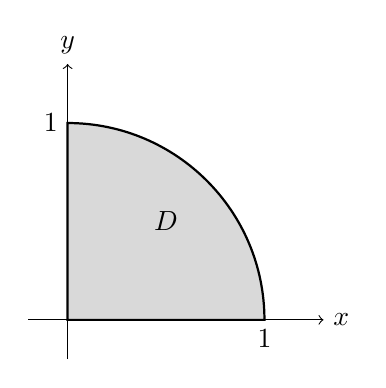
\begin{tikzpicture}[scale=2.5]
        \draw[->] (-0.2,0) -- (1.3,0) node[right] {$x$};
        \draw[->] (0,-0.2) -- (0,1.3) node[above] {$y$};
        \fill[gray!30] (0,0) -- (1,0) arc (0:90:1) -- cycle;
        \draw[thick] (0,0) -- (1,0) arc (0:90:1) -- cycle;
        \node[below] at (1,0) {$1$};
        \node[left] at (0,1) {$1$};
        \node at (0.5,0.5) {$D$};
    \end{tikzpicture}
    \end{center}

    这个区域其实是单位圆在第一象限的部分。被积函数 \(x^2+y^2=\rho^2\)，面积微元是 \(\rho\,d\rho\,d\theta\)。于是原积分变成极坐标下的累次积分：
    \[
    \int_0^{\frac{\pi}{2}}\left[\int_0^1 \rho^2\cdot \rho\,d\rho\right]d\theta
    = \int_0^{\frac{\pi}{2}}\left[\int_0^1 \rho^3\,d\rho\right]d\theta
    \]

    先对 \(\rho\) 积分：
    \[
    \int_0^1 \rho^3\,d\rho = \left[\frac{\rho^4}{4}\right]_0^1 = \frac14
    \]

    再对 \(\theta\) 积分：
    \[
    \int_0^{\frac{\pi}{2}} \frac14\,d\theta = \frac14\cdot\frac{\pi}{2} = \frac{\pi}{8}
    \]

    所以原积分 \(\int_0^1\left[\int_0^{\sqrt{1-x^2}} (x^2+y^2)\,dy\right]dx = \frac{\pi}{8}\)。
\end{myexample}

\begin{myexample}
    计算二重积分$\iint_D e^{x^2+y^2}\,d\sigma$，其中 $D$ 是由圆心在原点、半径为 $a$ 的圆周所围成的闭区域。

    被积函数有$e^{x^2+y^2}$，这是一个典型的“积不出”函数。但是我们可以通过极坐标把它积出来。

    令$x = \rho\cos\theta$，$y = \rho\sin\theta$，则：
\[
\iint_D e^{x^2+y^2}\,d\sigma = \iint_D e^{\rho^2}\,\rho d\rho d\theta
= \int_0^{2\pi} d\theta \int_0^a \rho e^{\rho^2} \,d\rho
\]

对 $\rho$ 积分，令 $u = \rho^2$，$du = 2\rho\,d\rho$，则：
\[
\int_0^a \rho e^{\rho^2}\,d\rho = \frac{1}{2} \int_0^{a^2} e^u\,du
= \frac{1}{2}(e^{a^2} - 1)
\]

再对 $\theta$ 积分：
\[
\int_0^{2\pi} \frac{1}{2}(e^{a^2} - 1)\, d\theta = 2\pi \cdot \frac{1}{2}(e^{a^2} - 1) =\pi(e^{a^2} - 1)
\]

所以
\(\iint_D e^{x^2+y^2}\,d\sigma
= \pi(e^{a^2} - 1)\)。
\end{myexample}

总结一下，用极坐标计算二重积分，先看被积函数和积分区域是否适合用极坐标，通常含有 \(x^2+y^2\)、\(\frac{y}{x}\) 这类式子，或者区域是圆、环、扇形等形状时，极坐标都是很好的选择。然后画出积分区域，用“画图穿线法”确定 \(\rho\) 的上下限和 \(\theta\) 的范围。射线从极点出发，穿入点作为 \(\rho\) 的下限，穿出点作为\(\rho\) 的上限，所有这样的射线扫过的角度范围就是 \(\theta\) 的积分区间。列式时切记面积微元是 $\textcolor{red}{\rho}d\rho d\theta$，不是$d\rho d\theta$。最后先 \(\rho\) 后 \(\theta\)化为累次积分，一步步算出来就行了。

\section{三重积分}
定积分和二重积分的定义可以很自然地扩展到三重积分。不过在进入三重积分之前，我们需要重新认识定积分和二重积分。
\subsection{三重积分}

在定积分和二重积分的定义里，我们总是将一点的函数值与我们要积分的微元相乘，比如定积分是函数值与线段微元相乘，二重积分是函数值与面积微元相乘。如果我们将函数值看成密度函数，那么我们就能用积分求质量。也就是说，对一个函数积分，就能得到积分区域的质量。

具体到定积分，就是已知细杆的线密度$f(x)$，积分求细杆质量。到了二重积分，就是已知薄板的面密度$f(x,y)$，积分求薄板质量。而我们生活在三维空间里，接触的都是空间体，仿照定积分和二重积分，如果我们已知物体的体密度$f(x,y,z)$，就能求出这个物体的质量了。这就是三重积分的物理意义。

在几何上，三重积分求的是四维空间中，以三维区域为底，三元函数$f(x,y,z)$为顶的四维曲顶柱体的“四维体积”。这很难想象，物理意义相比之下更直观也更容易理解。

仿照二重积分，我们再推广一步就能得到三重积分的定义。设 $w = f(x, y, z)$ 是定义在空间区域 $\Omega$ 上的函数。把 $\Omega$ 分成 $n$ 个小块$\Delta V_1,\ \Delta V_2,\ \cdots,\ \Delta V_n$，在每小块上取一点 $(\xi_i, \eta_i, \zeta_i)$，作和 $\sum_{i=1}^n f(\xi_i, \eta_i, \zeta_i)\, \Delta V_i$，取极限就得到三重积分。这本质上还是“分割、近似、求和、取极限”的思想。

\begin{definition}{三重积分}{}
设函数 \(f(x,y,z)\) 在有界闭区域 \(\Omega\) 上有界。将 \(\Omega\) 任意分成 \(n\) 个小闭区域
\[
\Delta V_1,\ \Delta V_2,\ \cdots,\ \Delta V_n
\]
每个小区域既表示该区域本身，也表示该区域的体积。在每个小区域 \(\Delta V_i\) 上任取一点 \((\xi_i,\eta_i,\zeta_i)\)，作函数值 \(f(\xi_i,\eta_i,\zeta_i)\) 与小区域体积 \(\Delta V_i\) 的乘积 \(f(\xi_i,\eta_i,\zeta_i) \cdot \Delta V_i\)，并作出和
\[
S = \sum_{i=1}^{n} f(\xi_i,\eta_i,\zeta_i) \Delta V_i
\]

记 \(d_i\) 为小区域 \(\Delta V_i\) 的直径，即该小区域内任意两点间距离的最大值，令 \(\lambda = \max\{d_1,d_2,\cdots,d_n\}\)。如果当 \(\lambda \to 0\) 时，\(S\) 的极限总存在，且与闭区域 \(\Omega\) 的分法及点 \((\xi_i,\eta_i,\zeta_i)\) 的取法无关，那么称 \(f(x,y,z)\) 在 \(\Omega\) 上\textbf{可积}，并称这个极限 \(I\) 为函数 \(f(x,y,z)\) 在闭区域 \(\Omega\) 上的\textbf{三重积分}，记作
\[
\iiint\limits_{\Omega} f(x,y,z)\,dV
\quad\text{或}\quad
\iiint\limits_{\Omega} f(x,y,z)\,dxdydz
\]
即：
\[
\iiint\limits_{\Omega} f(x,y,z)\,dV = \lim_{\lambda \to 0} \sum_{i=1}^{n} f(\xi_i,\eta_i,\zeta_i) \Delta V_i = I
\]

其中 \(f(x,y,z)\) 称为\textbf{被积函数}，\(f(x,y,z)\,dV\) 称为\textbf{被积表达式}，\(x,y,z\) 称为\textbf{积分变量}，\(\Omega\) 称为\textbf{积分区域}，$\iiint$称为\textbf{三重积分号}。
\end{definition}

一重积分切线段，二重积分切平面，三重积分切空间。积分号从 $\int$ 到 $\iint$ 到 $\iiint$，代表累加的维度越来越多。这个模式还可以继续推广到更高维。

三重积分的性质和二重积分完全一样。这里我们不再重复。


\begin{myexample}
  求 $\iiint_\Omega 2\, dV$，其中 $\Omega$ 是以原点为球心、半径为 $R$ 的球体。

  根据三重积分的物理意义，$\Omega$的体密度是$2$，也就是说这个球体密度处处为$2$。体积就是整个球体体积，那么质量就是$2\cdot \frac43 \pi R^3=\frac83 \pi R^3$。

所以$\iiint_\Omega 2\, dV=\frac83 \pi R^3$。
\end{myexample}

三重积分的定义直接用定义来计算不现实。我们需要像二重积分一样把它转化为累次积分才好计算。

\subsection{三重积分的直角坐标形式}

和二重积分类似，三重积分也是将积分化为一次次的定积分进行计算。三重积分的体积微元在直角坐标下就是 \(dV = dx\,dy\,dz\)，所以三重积分归根结底就是对 \(x,y,z\) 依次做定积分。不过具体按照什么顺序，就要看积分区域长什么样。一般我们有两种思路，一种是把空间区域投影到平面上，先穿一条线，再扫一个面。另一种是用垂直于某条坐标轴的平面去切，像切面包片，先把每片上的二重积分算出来，再把片累加起来。它们分别叫“投影法”和“截面法”。按照积分的顺序，它们又叫作“先一后二法”和“先二后一法”。

设空间区域 \(\Omega\) 在 \(xOy\) 平面上的投影为 \(D_{xy}\)，并且 \(\Omega\) 恰好夹在两张曲面之间，下方曲面是 \(z=z_1(x,y)\)，上方曲面是 \(z=z_2(x,y)\)，即：
\[
\Omega = \{(x,y,z) \mid (x,y)\in D_{xy},\; z_1(x,y) \le z \le z_2(x,y)\}
\]

我们依旧用“画图穿线法”确定上下限。先固定 \((x,y)\)，沿着$z$轴竖着穿一条线。这条线穿进 \(\Omega\) 里的地方就是下边界 \(z=z_1(x,y)\)，穿出去的地方是上边界 \(z=z_2(x,y)\)。先对 \(z\) 积分，积分下限就是\(z=z_1(x,y)\)，积分上限就是\(z=z_2(x,y)\)，积分得到这条“细杆”的累积量，然后把 \(D_{xy}\) 上所有的“细杆”加起来，也就是以区域\(D_{xy}\)做二重积分。最后就求得了三重积分的值。这就是投影法的思想。

\begin{theorem}{三重积分的投影法}{}
设空间闭区域 \(\Omega\) 可表示为
\[
\Omega = \{(x,y,z) \mid (x,y) \in D_{xy},\; z_1(x,y) \le z \le z_2(x,y)\}
\]
其中 \(D_{xy}\) 是 \(\Omega\) 在 \(xOy\) 面上的投影区域，\(z_1(x,y)\)，\(z_2(x,y)\) 在 \(D_{xy}\) 上连续。若 \(f(x,y,z)\) 在 \(\Omega\) 上可积，则
\[
\iiint_{\Omega} f(x,y,z)\,dxdydz
= \iint_{D_{xy}} \left( \int_{z_1(x,y)}^{z_2(x,y)} f(x,y,z)\,dz \right) dxdy
\]
\end{theorem}

这跟二重积分中“先穿一条线，再扫一个面”的做法一模一样，只不过现在多了一根 \(z\) 轴，线是竖着的，扫的是投影面\(D_{xy}\)。

用物理意义理解，就是根据密度函数求出了一条极细的“细杆”质量，然后做二重积分，求出所有这些“细杆”在“薄板”上的质量，这样就是整个空间体的质量。

\begin{center}
    \pgfmathdeclarefunction{F}{2}{%
  \pgfmathparse{1.05 + 0.22*#1 + 0.12*#2 + 0.32*sin(70*#1)}%
    }
\begin{tikzpicture}[
    scale=1.05,
    x={(1cm,0cm)},
    y={(0.55cm,0.32cm)},
    z={(0cm,1cm)},
    line join=round,
    line cap=round
]
    % 椭圆形底域 D 的参数
    \def\cx{2.15}
    \def\cy{1.15}
    \def\ra{1.55}
    \def\rb{0.78}

    % 坐标轴
    \draw[->] (-0.25,0,0) -- (4.45,0,0) node[below] {$x$};
    \draw[->] (0,-0.2,0) -- (0,2.85,0) node[right] {$y$};
    \draw[->] (0,0,0) -- (0,0,3.8) node[left] {$z$};
    \node[below left] at (0,0,0) {$O$};

    

    % 侧面 —— 用不透明的浅色填充，不加渐变
    \fill[cyan!20]   % 不透明，颜色自行调整
        plot[domain=0:360, samples=120, smooth]
        ({\cx + \ra*cos(\x)}, {\cy + \rb*sin(\x)},
         {F(\cx + \ra*cos(\x), \cy + \rb*sin(\x)) + 1})
        -- plot[domain=360:0, samples=120, smooth]
        ({\cx + \ra*cos(\x)}, {\cy + \rb*sin(\x)}, 1)
        -- cycle;

    % 母线 —— 用虚线表达柱面的弯曲，无光照感
    \foreach \ang in {0,1,...,359} {
        \pgfmathsetmacro\xx{\cx + \ra*cos(\ang)}
        \pgfmathsetmacro\yy{\cy + \rb*sin(\ang)}
        \pgfmathsetmacro\zz{F(\xx,\yy)}
        \draw[cyan!40, line width=0.4mm] (\xx,\yy,1) -- (\xx,\yy,\zz+1);
    }

    % 曲顶 z = f(x,y) + 1
    \fill[blue!18, opacity=0.72]
        plot[domain=0:360, samples=120, smooth]
        ({\cx + \ra*cos(\x)}, {\cy + \rb*sin(\x)},
         {F(\cx + \ra*cos(\x), \cy + \rb*sin(\x)) + 1})
        -- cycle;

    % 底域 D（浅色填充，不透明）
    \draw[cyan!70!black, thick]
        plot[domain=195:360, samples=80, smooth]
        ({\cx + \ra*cos(\x)}, {\cy + \rb*sin(\x)}, 1);

    \draw[cyan!70!black, thick, dashed]
        plot[domain=0:195, samples=80, smooth]
        ({\cx + \ra*cos(\x)}, {\cy + \rb*sin(\x)}, 1);

    % 底面与顶面的轮廓线
    \draw[blue!75!black, very thick]
        plot[domain=0:360, samples=120, smooth]
        ({\cx + \ra*cos(\x)}, {\cy + \rb*sin(\x)},
         {F(\cx + \ra*cos(\x), \cy + \rb*sin(\x)) + 1});

         \draw[red!70!black, thick]
        plot[domain=0:360, samples=80, smooth]
        ({\cx + \ra*cos(\x)}, {\cy + \rb*sin(\x)}, 0);

        \fill [red!24!white,opacity=0.72]
        plot[domain=0:360, samples=120, smooth] ({\cx + \ra*cos(\x)}, {\cy + \rb*sin(\x)}, 0) -- cycle;
        
    \draw[thick] (2.15,1.15,2.82) -- (2.15,1.15,3.62);
    \draw[thick] (2.15,1.15,-0.1) -- (2.15,1.15,0.75);
    \draw[thick,dashed] (2.15,1.15,0.75) -- (2.15,1.15,2.82);

    
    \node[blue!70!black, above] at (3.2,1.4,1) {$\Omega$};
    \node[red!70!black, above] at (3.2,1.4,0) {$D_{xy}$};

    % ----- 引线标注 -----
    % 顶面标注：从右上方引线指向曲面
    \draw[thick]
        (4.0, 2.3, {F(3.4,1.65)+1}) node[right] {$z_2=z_2(x,y)$}
        -- (3.4, 1.65, {F(3.4,1.65)+1});

    % 底面标注：从右侧引线指向底域 D
    \draw[thick]
    (5.2, 0.2, 1.1) node[right] {$z_1=z_1(x,y)$}
    -- (3.692, 1.223, 1);
\end{tikzpicture}
\end{center}

当然，投影不一定非要投到 \(xOy\) 面，根据区域\(\Omega\)形状，投到 \(xOz\) 面或 \(yOz\) 面也一样，道理不变。

如果沿着某条轴看过去，区域 \(\Omega\) 的截面形状特别简单，那就更省事了。比如用垂直于 \(z\) 轴的平面 \(z = k\)（$k$为常数）去截 \(\Omega\)，截出来一个平面区域 \(D_z\)。先固定 \(z\)，在 \(D_z\) 上对 \(x,y\) 做二重积分，得到这一薄片的累积量，然后把所有薄片从 \(z=c\) 积到 \(z=d\)。这就是截面法的思想。

\begin{theorem}{三重积分的截面法}{}
设空间闭区域 \(\Omega\) 夹在平面 \(z = c\) 与 \(z = d\) 之间（\(c < d\)），对于每个 \(z \in [c,d]\)，用平面 \(z = k\)（$k$为常数）截 \(\Omega\) 所得的截面区域为 \(D_z\)。若 \(f(x,y,z)\) 在 \(\Omega\) 上可积，则
\[
\iiint_{\Omega} f(x,y,z)\,dxdydz
= \int_{c}^{d} \left( \iint_{D_z} f(x,y,z)\,dxdy \right) dz
\]
\end{theorem}

\begin{center}
    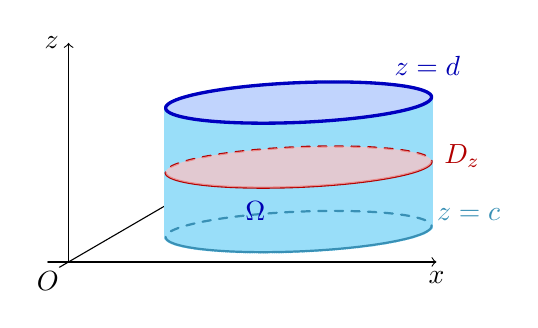
\begin{tikzpicture}[
        scale=1.05,
        x={(1cm,0cm)},
        y={(0.55cm,0.32cm)},
        z={(0cm,1cm)},
        line join=round,
        line cap=round
    ]
        % 椭圆形底域 D 的参数
        \def\cx{2.15}
        \def\cy{1.15}
        \def\ra{1.55}
        \def\rb{0.78}
        \def\H{1.56}   % 椭圆柱的高度（常数）

        % 坐标轴
        \draw[->] (-0.25,0,0) -- (4.45,0,0) node[below] {$x$};
        \draw[->] (0,-0.2,0) -- (0,2.85,0) node[right] {$y$};
        \draw[->] (0,0,0) -- (0,0,2.65) node[left] {$z$};
        \node[below left] at (0,0,0) {$O$};

        % 侧面 —— 用不透明的浅色填充，顶部高度为常数 \H
        \fill[cyan!20]
            plot[domain=0:360, samples=120, smooth]
            ({\cx + \ra*cos(\x)}, {\cy + \rb*sin(\x)}, \H)
            -- plot[domain=360:0, samples=120, smooth]
            ({\cx + \ra*cos(\x)}, {\cy + \rb*sin(\x)}, 0)
            -- cycle;

        % 母线 —— 用虚线表达柱面的棱边
        \foreach \ang in {0,1,...,359} {
            \pgfmathsetmacro\xx{\cx + \ra*cos(\ang)}
            \pgfmathsetmacro\yy{\cy + \rb*sin(\ang)}
            \draw[cyan!40, line width=0.4mm] (\xx,\yy,0) -- (\xx,\yy,\H);
        }

        % 顶面（平面 z = \H）
        \fill[blue!18, opacity=0.72]
            plot[domain=0:360, samples=120, smooth]
            ({\cx + \ra*cos(\x)}, {\cy + \rb*sin(\x)}, \H)
            -- cycle;

        % 底域 D 的轮廓（可见部分实线，不可见部分虚线）
        \draw[cyan!70!black, thick]
            plot[domain=195:360, samples=80, smooth]
            ({\cx + \ra*cos(\x)}, {\cy + \rb*sin(\x)}, 0);
        \draw[cyan!70!black, thick, dashed]
            plot[domain=0:195, samples=80, smooth]
            ({\cx + \ra*cos(\x)}, {\cy + \rb*sin(\x)}, 0);

        % 顶面轮廓线
        \draw[blue!75!black, very thick]
            plot[domain=0:360, samples=120, smooth]
            ({\cx + \ra*cos(\x)}, {\cy + \rb*sin(\x)}, \H);

        % 标签
        \node[blue!70!black, above] at (3.35,1.8,\H) {$z=d$};
        \node[blue!70!black, above] at (1.6,1.2,0) {$\Omega$};
        \node[cyan!70!black, right] at (3.35,1.8,0) {$z=c$};

        % 红色的截面 D_z（位于 z=0.78，可根据需要调整）
        \draw[red!70!black, thick]
            plot[domain=195:360, samples=80, smooth]
            ({\cx + \ra*cos(\x)}, {\cy + \rb*sin(\x)}, 0.78);
        \draw[red!70!black, thick, dashed]
            plot[domain=0:195, samples=80, smooth]
            ({\cx + \ra*cos(\x)}, {\cy + \rb*sin(\x)}, 0.78);
        \fill[red!24!white, opacity=0.72]
            plot[domain=0:360, samples=120, smooth]
            ({\cx + \ra*cos(\x)}, {\cy + \rb*sin(\x)}, 0.78) -- cycle;
        \node[red!70!black] at (4.76,0,1.28) {$D_z$};
    \end{tikzpicture}
\end{center}

当被积函数只和 \(z\) 有关，或者截面面积很容易写出来的时候，截面法往往比投影法简洁得多。

仔细观察我们发现，投影法是先对一个变量积分，再对两个变量积分，所以投影法又叫“先一后二法”。截面法是先对两个变量积分，再对一个变量积分，所以截面法又叫“先二后一法”。

下面看一个例子具体运用这两种方法。

\begin{myexample}
计算三重积分 \(\ \iiint_{\Omega} z\,dV\)，其中 \(\Omega\) 是由平面 \(x=0,\;y=0,\;z=0\) 以及 \(x+y+z=1\) 所围成的四面体。

区域\(\Omega\)是第一卦限里被坐标面切出来的一个四面体。我们先用投影法，把它投到 \(xOy\) 面上。投影区域 \(D\) 就是直线 \(x+y=1\) 与 \(x\) 轴、\(y\) 轴围成的三角形。

\begin{center}
    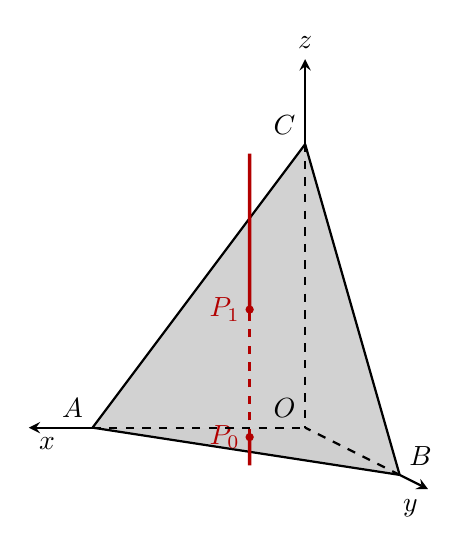
\begin{tikzpicture}[
        scale=3,
        line join=round,
        x={(-0.9cm,0cm)},
    y={(0.4cm,-0.2cm)},
    z={(0cm,1.2cm)},
        % 面样式
        bottom/.style={fill=gray!50,fill opacity=0.5},
        side/.style={fill=gray!50,fill opacity=0.4},
        slant/.style={fill=gray!50,fill opacity=0.5},
        edge/.style={thick},
    ]
    
    % 定义顶点
    \coordinate (O) at (0,0,0);
    \coordinate (A) at (1,0,0);
    \coordinate (B) at (0,1,0);
    \coordinate (C) at (0,0,1);
    
    % 填充各个面（半透明，所有棱都可见）
    \fill[bottom] (O) -- (A) -- (B) -- cycle;       % z=0 底面
    \fill[side]   (O) -- (A) -- (C) -- cycle;       % y=0 面
    \fill[side]   (O) -- (B) -- (C) -- cycle;       % x=0 面
    \fill[slant]  (A) -- (B) -- (C) -- cycle;       % x+y+z=1 斜面
    
    % 绘制所有棱
    \draw[edge] (A) -- (B);
    \draw[edge] (A) -- (C);
    \draw[edge] (B) -- (C);
    
    % 顶点标签
    \node [above left] at (O) {$O$};
    \node [above left] at (A) {$A$};
    \node [above right] at (B) {$B$};
    \node [above left] at (C) {$C$};

    \def\px{0.35}                     % 选取 x 坐标
    \def\py{0.2}                     % 选取 y 坐标
    \pgfmathsetmacro\pz{1-\px-\py}   % 计算上端点 z 坐标
    \coordinate (P0) at (\px,\py,0);
    \coordinate (P1) at (\px,\py,\pz);
    % 画穿线（带箭头）
    \draw[red!70!black, line width=1.2pt] (0.35,0.2,-0.1) -- (P0);
    \draw[red!70!black, line width=1.2pt,dashed] (P0) -- (P1);
    \draw[red!70!black, line width=1.2pt] (P1) -- (0.35,0.2,1);

    \fill[red!70!black] (P0) circle (0.5pt);
    \fill[red!70!black] (P1) circle (0.5pt);

    \node[left, red!70!black] at (P0) {$P_0$};
    \node[left, red!70!black] at (P1) {$P_1$};
    
    % 坐标轴（可选）
    \draw[-stealth,thick] (1,0,0) -- (1.3,0,0) node[below right] {$x$};
    \draw[-stealth,thick] (0,1,0) -- (0,1.3,0) node[below left] {$y$};
    \draw[-stealth,thick] (0,0,1) -- (0,0,1.3) node[above] {$z$};
    \draw[dashed,thick] (1,0,0) -- (O);
    \draw[dashed,thick] (0,1,0) -- (O);
    \draw[dashed,thick] (0,0,1) -- (O);
    \end{tikzpicture}
    \qquad
    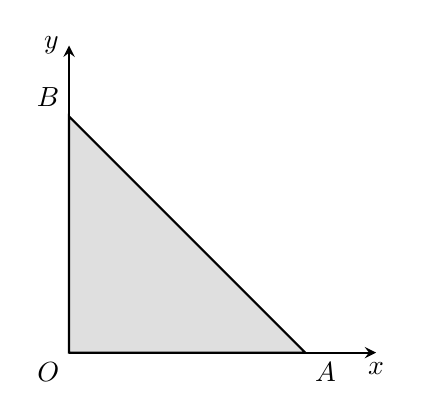
\begin{tikzpicture}[scale=3]
    % 填充投影区域（灰色半透明）
    \fill[gray!50, opacity=0.5] (0,0) -- (1,0) -- (0,1) -- cycle;
    % 边界
    \draw[thick] (0,0) -- (1,0) -- (0,1) -- cycle;
    % 顶点
    \node at (0,0)[below left] {$O$};
    \node at (1,0)[below right] {$A$};
    \node at (0,1)[above left] {$B$};
    % 坐标轴
    \draw[-stealth, thick] (0,0) -- (1.3,0) node[below] {$x$};
    \draw[-stealth, thick] (0,0) -- (0,1.3) node[left] {$y$};
\end{tikzpicture}
\end{center}

我们用“画图穿线法”沿着 \(z\) 轴方向穿线，从底面 \(z=0\) 进入，从平面 \(z = 1-x-y\) 穿出，交点分别是$P_0$，$P_1$。所以：
\[
\iiint_{\Omega} z\,dV
= \iint_{D} \left( \int_{0}^{1-x-y} z \, dz \right) dxdy
\]

内层对 \(z\) 积分时 \(x,y\) 是常数，积出来就是 \(\frac12(1-x-y)^2\)。于是原积分化成二重积分：
\[
\iiint_{\Omega} z\,dV = \iint_{D} \frac12(1-x-y)^2\,dxdy
= \frac12 \int_{0}^{1} dx \int_{0}^{1-x} (1-x-y)^2\,dy
\]

先对 \(y\) 积分：
\[
\int_{0}^{1-x} (1-x-y)^2\,dy
= \left[ -\frac13 (1-x-y)^3 \right]_{0}^{1-x}
= \frac13 (1-x)^3
\]

再对 \(x\) 积分：
\[
\frac12 \cdot \frac13 \int_{0}^{1} (1-x)^3\,dx
= \frac16 \left[ -\frac14 (1-x)^4 \right]_{0}^{1}
= \frac16 \cdot \frac14 = \frac{1}{24}
\]

所以 \(\iiint_{\Omega} z\,dV = \frac{1}{24}\)。

再用截面法，用平面 \(z = k\)（$k$为常数）截 \(\Omega\)，我们能得到一个等腰直角三角形，这个等腰直角三角形的边长随\(z\)的变化而变化。由于截面上的点在区域\(\Omega\)内部，所以它们满足\(x+y+z\le1\)，也就是\(x+y\le1-z\)，这说明等腰直角三角形的边长就是\(1-z\)。

\begin{center}
    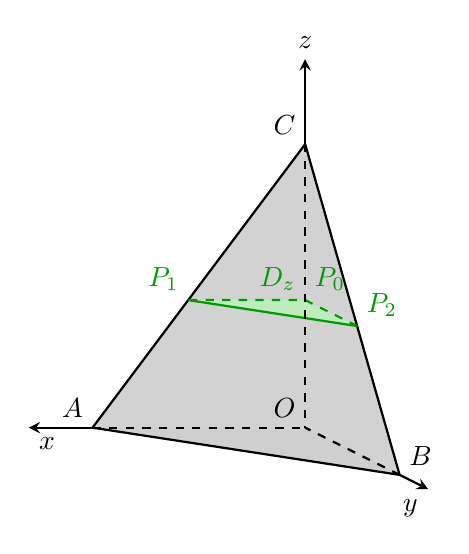
\begin{tikzpicture}[
        scale=3,
        line join=round,
        x={(-0.9cm,0cm)},
        y={(0.4cm,-0.2cm)},
        z={(0cm,1.2cm)},
        % 面样式
        bottom/.style={fill=gray!50,fill opacity=0.5},
        side/.style={fill=gray!50,fill opacity=0.4},
        slant/.style={fill=gray!50,fill opacity=0.5},
        edge/.style={thick},
    ]
    
    % 定义顶点
    \coordinate (O) at (0,0,0);
    \coordinate (A) at (1,0,0);
    \coordinate (B) at (0,1,0);
    \coordinate (C) at (0,0,1);
    
    % 填充各个面（半透明，所有棱都可见）
    \fill[bottom] (O) -- (A) -- (B) -- cycle;       % z=0 底面
    \fill[side]   (O) -- (A) -- (C) -- cycle;       % y=0 面
    \fill[side]   (O) -- (B) -- (C) -- cycle;       % x=0 面
    \fill[slant]  (A) -- (B) -- (C) -- cycle;       % x+y+z=1 斜面
    
    % 绘制所有棱
    \draw[edge] (A) -- (B);
    \draw[edge] (A) -- (C);
    \draw[edge] (B) -- (C);
    
    \def\px{0.35}                     % 选取 x 坐标
    \def\py{0.2}                     % 选取 y 坐标
    \pgfmathsetmacro\pz{1-\px-\py}   % 截面高度：与穿线终点一致 (0.45)
    % 截面三角形顶点 (在高度 z = \pz 处)
    \coordinate (Dz0) at (0,0,\pz);
    \coordinate (Dz1) at ({1-\pz},0,\pz);
    \coordinate (Dz2) at (0,{1-\pz},\pz);
    % 绘制截面（半透明绿色填充，边界线加粗）
    \fill[green!30, opacity=0.6] (Dz0) -- (Dz1) -- (Dz2) -- cycle;
    \draw[green!60!black, thick, dashed] (Dz2) -- (Dz0) -- (Dz1);
    \draw[green!60!black, thick] (Dz2) -- (Dz1);
    % 标签
    \node[green!60!black, above left] at (0,0,\pz) {$D_z$};
    
    \node[green!60!black, above right] at (Dz0) {$P_0$};
    \node[green!60!black, above left] at (Dz1) {$P_1$};
    \node[green!60!black, above right] at (Dz2) {$P_2$};

    % 顶点标签
    \node [above left] at (O) {$O$};
    \node [above left] at (A) {$A$};
    \node [above right] at (B) {$B$};
    \node [above left] at (C) {$C$};


    % 坐标轴
    \draw[-stealth,thick] (1,0,0) -- (1.3,0,0) node[below right] {$x$};
    \draw[-stealth,thick] (0,1,0) -- (0,1.3,0) node[below left] {$y$};
    \draw[-stealth,thick] (0,0,1) -- (0,0,1.3) node[above] {$z$};
    \draw[dashed,thick] (1,0,0) -- (O);
    \draw[dashed,thick] (0,1,0) -- (O);
    \draw[dashed,thick] (0,0,1) -- (O);
    \end{tikzpicture}
    \qquad
    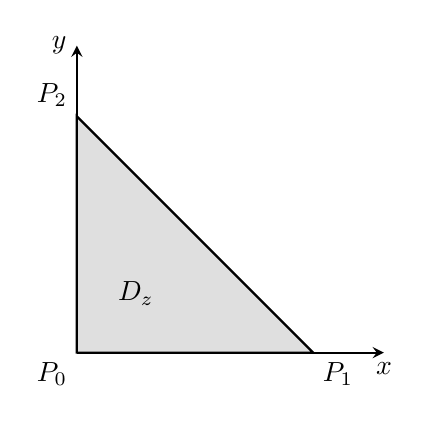
\begin{tikzpicture}[scale=3]
    % 填充投影区域（灰色半透明）
    \fill[gray!50, opacity=0.5] (0,0) -- (1,0) -- (0,1) -- cycle;
    % 边界
    \draw[thick] (0,0) -- (1,0) -- (0,1) -- cycle;
    % 顶点
    \node at (0,0)[below left] {$P_0$};
    \node at (1,0)[below right] {$P_1$};
    \node at (0,1)[above left] {$P_2$};
    \node at (0.25,0.25) {$D_z$};
    % 坐标轴
    \draw[-stealth, thick] (0,0) -- (1.3,0) node[below] {$x$};
    \draw[-stealth, thick] (0,0) -- (0,1.3) node[left] {$y$};
    \end{tikzpicture}
\end{center}

所以截面\(D_z\)的面积为\(\frac12 (1-z)^2\)。先对截面积分，即：
\[
\iiint_{\Omega} z\,dV
= \int_{0}^{1} \left( \iint_{D_z} z\,dxdy \right) dz
\]

二重积分里对\(x,y\)积分，因此\(z\)是常数。把\(z\)提出来，就是：
\[
\int_{0}^{1} \left( \iint_{D_z} z\,dxdy \right) dz=\int_{0}^{1} z \left( \iint_{D_z} \,dxdy \right) dz=\int_{0}^{1} [z\cdot\frac12 (1-z)^2] \,dz
\]

所以：
\[
\int_{0}^{1} [z\cdot\frac12 (1-z)^2] \,dz
= \frac12 \int_{0}^{1} \bigl( z - 2z^2 + z^3 \bigr) \, dz
= \frac12 \left[ \frac{z^2}{2} - \frac{2z^3}{3} + \frac{z^4}{4} \right]_{0}^{1}
= \frac12 (\frac12 - \frac23 + \frac14)
= \frac{1}{24}
\]

所以 \(\iiint_{\Omega} z\,dV = \frac{1}{24}\)。
\end{myexample}

\begin{myexample}
计算三重积分 \(\iiint_{\Omega} z\,dV\)，其中 \(\Omega\) 是由圆锥面 \(z = \sqrt{x^2+y^2}\) 与平面 \(z = 1\) 所围成的区域。

我们用截面法计算这个积分。用垂直于 \(z\) 轴的平面去截这个区域，所得的截面都是圆。圆的半径随\(z\)的变化而变化，对于 \(z \in [0,1]\)，截面 \(D_z\) 是圆 \(x^2+y^2 \le z^2\)，面积就是 \(\pi z^2\)。

\begin{center}
    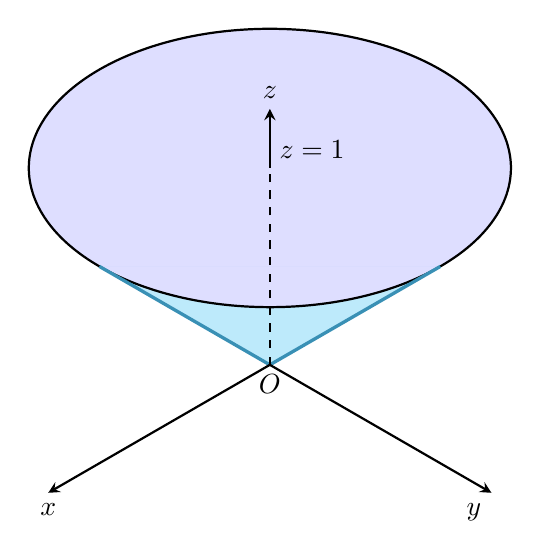
\begin{tikzpicture}[
        scale=2.5,
        line join=round,
        % 视角调整：使顶点在下，底面在上
        x={(-0.866cm,-0.5cm)},
        y={(0.866cm,-0.5cm)},
        z={(0cm,1cm)},
    ]
    
    % 圆锥参数
    \def\R{1}    % 底面半径
    \def\H{1}    % 高度
    
    % 顶点与底面圆心
    \coordinate (V) at (0,0,0);
    \coordinate (Otop) at (0,0,\H);
    
    
    \fill[cyan!40, opacity=0.65, even odd rule]
        (V) -- ({\R*cos(0)}, {\R*sin(0)}, \H) -- ({\R*cos(90)}, {\R*sin(90)}, \H) -- cycle
        % 弓形：从 A 沿弧到 B，再 -- cycle 闭合（弦 BA）
        plot[domain=0:90, samples=120, variable=\t, smooth]
            ({\R*cos(\t)}, {\R*sin(\t)}, \H)
        -- cycle;
    
    % ---- 顶面（半透明填充） ----
    \fill[blue!20, opacity=0.65]
        plot[domain=0:360, samples=120, smooth]
        ({\R*cos(\x)}, {\R*sin(\x)}, \H) -- cycle;
    
    % ---- 底面圆的轮廓线 ----
    \draw[thick]
        plot[domain=0:360, samples=120, smooth]
        ({\R*cos(\x)}, {\R*sin(\x)}, \H);
    
    
    \draw[very thick, cyan!70!black] (V) -- ({\R*cos(0)}, {\R*sin(0)}, \H);
    
    \draw[very thick, cyan!70!black] (V) -- ({\R*cos(90)}, {\R*sin(90)}, \H);
    
    
    % ---- 坐标轴（从顶点向外延伸） ----
    \draw[-stealth, thick] (V) -- (1.3,0,0) node[below] {$x$};
    \draw[-stealth, thick] (V) -- (0,1.3,0) node[below left] {$y$};
    \draw[-stealth, thick] (0,0,1) -- (0,0,1.3) node[above] {$z$};
    \draw[thick, dashed] (V) -- (0,0,1);
    
    % 标签
    \node[below] at (V) {$O$};
    \node[above right] at (0,0,\H) {$z=1$};
    
    \end{tikzpicture}
    \quad
    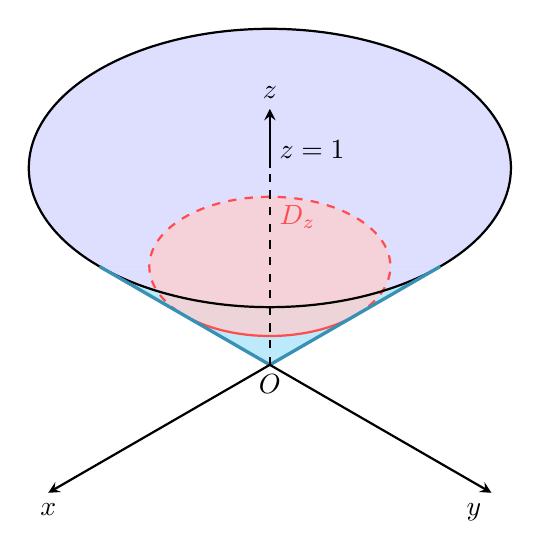
\begin{tikzpicture}[
    scale=2.5,
    line join=round,
    % 视角调整：使顶点在下，底面在上
    x={(-0.866cm,-0.5cm)},
    y={(0.866cm,-0.5cm)},
    z={(0cm,1cm)},
]

% 圆锥参数
\def\R{1}    % 底面半径
\def\H{1}    % 高度

% 顶点与底面圆心
\coordinate (V) at (0,0,0);
\coordinate (Otop) at (0,0,\H);


\fill[cyan!40, opacity=0.65, even odd rule]
    (V) -- ({\R*cos(0)}, {\R*sin(0)}, \H) -- ({\R*cos(90)}, {\R*sin(90)}, \H) -- cycle
    % 弓形：从 A 沿弧到 B，再 -- cycle 闭合（弦 BA）
    plot[domain=0:90, samples=120, variable=\t, smooth]
        ({\R*cos(\t)}, {\R*sin(\t)}, \H)
    -- cycle;

% ---- 顶面（半透明填充） ----
\fill[blue!20, opacity=0.65]
    plot[domain=0:360, samples=120, smooth]
    ({\R*cos(\x)}, {\R*sin(\x)}, \H) -- cycle;

    \fill[red!20, opacity=0.72]
    plot[domain=0:360, samples=120, smooth]
    ({0.5*\R*cos(\x)}, {0.5*\R*sin(\x)}, 0.5) -- cycle;
    
    \draw[red!70, thick]
    plot[domain=0:90, samples=120, smooth]
    ({0.5*\R*cos(\x)}, {0.5*\R*sin(\x)}, 0.5);

    \draw[red!70, thick, dashed]
    plot[domain=90:360, samples=120, smooth]
    ({0.5*\R*cos(\x)}, {0.5*\R*sin(\x)}, 0.5);

    \node[red!70, right] at (0,0,0.75) {$D_z$};

% ---- 底面圆的轮廓线 ----
\draw[thick]
    plot[domain=0:360, samples=120, smooth]
    ({\R*cos(\x)}, {\R*sin(\x)}, \H);


\draw[very thick, cyan!70!black] (V) -- ({\R*cos(0)}, {\R*sin(0)}, \H);

\draw[very thick, cyan!70!black] (V) -- ({\R*cos(90)}, {\R*sin(90)}, \H);


% ---- 坐标轴（从顶点向外延伸） ----
\draw[-stealth, thick] (V) -- (1.3,0,0) node[below] {$x$};
\draw[-stealth, thick] (V) -- (0,1.3,0) node[below left] {$y$};
\draw[-stealth, thick] (0,0,1) -- (0,0,1.3) node[above] {$z$};
\draw[thick, dashed] (V) -- (0,0,1);

% 标签
\node[below] at (V) {$O$};
\node[above right] at (0,0,\H) {$z=1$};


\end{tikzpicture}
\end{center}

被积函数只含 \(z\)，所以：
\[
\iiint_{\Omega} z\,dV
= \int_{0}^{1} z \left( \iint_{D_z} dxdy \right) dz
\]

已知截面面积为 \(\pi z^2\)，代入二重积分，得：
\[
\int_{0}^{1} z \left( \iint_{D_z} dxdy \right) dz
= \int_{0}^{1} z \cdot \pi z^2 \, dz
= \pi \int_{0}^{1} z^3\,dz
= \frac{\pi}{4}
\]

所以 \( \iiint_{\Omega} z\,dV = \frac{\pi}{4}\)。
\end{myexample}

总的来说，直角坐标下算三重积分，关键的是先看清区域的形状，选择合适的方法。投影法投到平面再穿线，和算二重积分思路十分相似。截面法像切面包片，用垂直于 \(z\) 轴的平面去截区域，然后计算截面面积，可以理解为升维的“画图穿线法”。

\subsection{三重积分的柱面坐标形式}

在研究二重积分时我们发现，当积分区域是圆、环或扇形，或者被积函数含有 \(x^2+y^2\) 这类项时，用极坐标往往能大大简化计算。在三重积分里，类似的场景也会出现。如果空间区域 \(\Omega\) 在某个平面上的投影是圆形或扇形区域，而被积函数又含有 \(x^2+y^2\) 之类的项，那么就可以考虑用柱面坐标。

柱面坐标其实就是平面极坐标加上一个竖坐标 \(z\)。我们知道，在平面上确定一个点可以用极坐标 \((\rho,\theta)\)，那么在空间中，要确定一个点，只需要在 \((\rho,\theta)\) 的基础上再给出它的竖坐标 \(z\) 就可以了。也就是说，空间中一点 \(M\) 的柱面坐标是 \((\rho,\theta,z)\)，其中 \(0\le \rho<+\infty\)，\(0\le|\theta|\le 2\pi\)，\(-\infty<z<+\infty\)。

\begin{center}
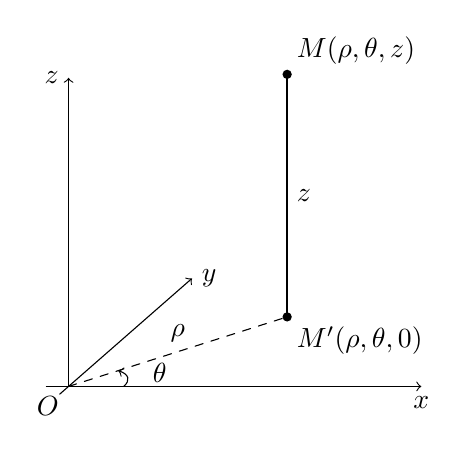
\begin{tikzpicture}[
    scale=1.4,
    x={(1cm,0cm)},
    y={(0.4cm,0.35cm)},
    z={(0cm,1cm)},
    line join=round,
    line cap=round
]
    % 坐标轴
    \draw[->] (-0.2,0,0) -- (3.2,0,0) node[below] {$x$};
    \draw[->] (0,-0.2,0) -- (0,2.8,0) node[right] {$y$};
    \draw[->] (0,0,0) -- (0,0,2.8) node[left] {$z$};
    \node[below left] at (0,0,0) {$O$};

    % 定义点 P 的坐标
    \def\rr{2.2}
    \def\th{55}
    \def\zz{2.2}

    % 计算点 P 的直角坐标
    \pgfmathsetmacro\xx{\rr*cos(\th)}
    \pgfmathsetmacro\yy{\rr*sin(\th)}

    % 点 P
    \coordinate (P) at (\xx,\yy,\zz);
    \fill (P) circle (1.2pt) node[above right] {$M(\rho,\theta,z)$};

    % 投影点 P' 在 xOy 平面上
    \coordinate (Pxy) at (\xx,\yy,0);
    \fill (Pxy) circle (1.2pt) node[below right] {$M'(\rho,\theta,0)$};

    % 连接
    \draw[dashed] (P) -- (Pxy);
    \draw[dashed] (0,0,0) -- (Pxy);

    % 标出 z
    \draw[thick] (\xx,\yy,0) -- (\xx,\yy,\zz);
    \node[right] at (\xx,\yy,\zz/2) {$z$};

    % 标出 rho
    \node[above] at (\xx/2,\yy/2,0) {$\rho$};

    % 标出 theta 角
    \draw[->] (0.5,0,0) arc (0:\th:0.5);
    \node[right] at (0.54,0.34,0) {$\theta$};

\end{tikzpicture}
\end{center}

也就是说，柱面坐标与极坐标之间的关系只不过是多了竖坐标 \(z\) ，那么直角坐标转换为柱面坐标也就和极坐标类似：
\[
x = \rho\cos\theta,\quad
y = \rho\sin\theta,\quad
z = z
\]

那么柱面坐标下的体积微元是什么形式呢？回忆二重极坐标的面积微元，是用无数多个同心圆和无数条从原点出发的射线把平面分割成小网格，每个小网格近似为一个“曲边矩形”，边长分别是 \(\Delta \rho\) 和 \(\rho\Delta\theta\)，面积近似为 \(\rho\,\Delta \rho\,\Delta\theta\)，取极限得到 \(d\sigma = \rho\,d\rho\,d\theta\)。

\begin{center}
    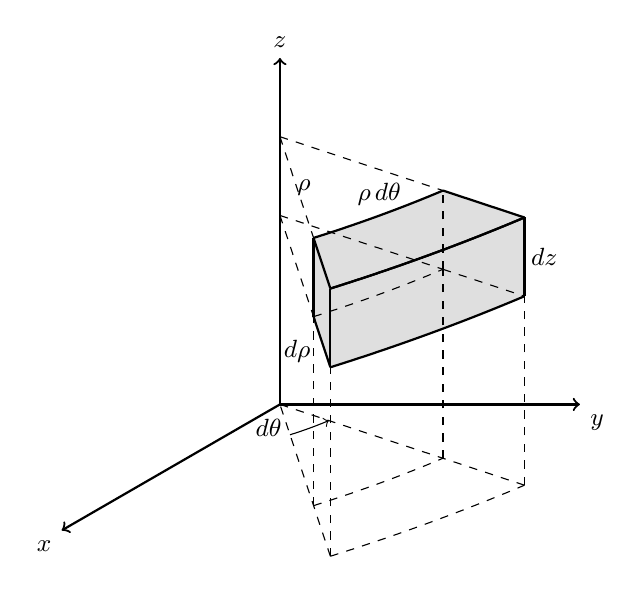
\begin{tikzpicture}[
        x={(-0.866cm, -0.5cm)},
        y={(0.866cm, 0cm)},
        z={(0cm, 1cm)},
        scale=2,
        font=\small
    ]
    
    % ---------- 几何参数 ----------
    \def\myr{2}       % 内径
    \def\mydr{1}      % 径向增量
    \def\dtheta{20}   % 角度增量（度）
    \def\z{1.2}         % 底面高度
    \def\dz{0.5}      % 高度增量
    
    % 外径
    \pgfmathtruncatemacro{\myR}{\myr+\mydr}
    
    % 起止角度（使微元在视角下对称一些）
    \pgfmathsetmacro{\thetaStart}{-0.5*\dtheta+60}
    \pgfmathsetmacro{\thetaEnd}{0.5*\dtheta+60}
    
    % ---------- 关键点坐标 ----------
    % 底面内圆柱面端点
    \coordinate (A) at ({\myr*cos(\thetaStart)}, {\myr*sin(\thetaStart)}, \z);
    \coordinate (B) at ({\myr*cos(\thetaEnd)},   {\myr*sin(\thetaEnd)},   \z);
    % 底面外圆柱面端点
    \coordinate (C) at ({\myR*cos(\thetaStart)}, {\myR*sin(\thetaStart)}, \z);
    \coordinate (D) at ({\myR*cos(\thetaEnd)},   {\myR*sin(\thetaEnd)},   \z);
    % 顶面内圆柱面端点
    \coordinate (E) at ({\myr*cos(\thetaStart)}, {\myr*sin(\thetaStart)}, \z+\dz);
    \coordinate (F) at ({\myr*cos(\thetaEnd)},   {\myr*sin(\thetaEnd)},   \z+\dz);
    % 顶面外圆柱面端点
    \coordinate (G) at ({\myR*cos(\thetaStart)}, {\myR*sin(\thetaStart)}, \z+\dz);
    \coordinate (H) at ({\myR*cos(\thetaEnd)},   {\myR*sin(\thetaEnd)},   \z+\dz);
    
    \fill[gray!50,opacity=0.5] 
      (E) arc[start angle=\thetaStart, end angle=\thetaEnd, radius=\myr] 
      -- (H) -- (D) arc[start angle=\thetaEnd, end angle=\thetaStart, radius=\myR] -- (A)
      -- cycle;
    
    % ---------- 绘制线框 ----------
    % 底面
    \draw[dashed]    (A) arc[start angle=\thetaStart, end angle=\thetaEnd, samples=120, radius=\myr];
    \draw[thick]     (C) arc[start angle=\thetaStart, end angle=\thetaEnd, samples=120, radius=\myR];
    \draw[thick]    (A) -- (C);
    \draw[dashed]     (B) -- (D);
    
    % 顶面
    \draw[thick]    (E) arc[start angle=\thetaStart, end angle=\thetaEnd, samples=120, radius=\myr];
    \draw[thick]     (G) arc[start angle=\thetaStart, end angle=\thetaEnd, samples=120, radius=\myR];
    \draw[thick]     (E) -- (G);
    \draw[thick]     (F) -- (H);
    
    % 侧棱
    \draw[thick] (A) -- (E);
    \draw[dashed] (B) -- (F);
    
    
    
    % ---------- 尺寸标注 ----------
    % dz（沿竖棱）
    \draw[thick] (D) -- (H) 
        node[midway, right=2pt, inner sep=0] {$dz$};
    
    % d\rho（沿径向外表面）
    \draw[thick] (C) -- (G) 
        node[midway, left=12pt, below=2pt, inner sep=2pt] {$d\rho$};
    
    % \rho d\theta（沿顶面外圆弧）
    \draw[thick] 
        (G) arc[start angle=\thetaStart, end angle=\thetaEnd, radius=\myR, samples=120] 
        node[midway, above=22pt, left=10pt, inner sep=0] {$\rho\,d\theta$};
    
        \draw[->] ({0.3*\myr*cos(\thetaStart)},{0.3*\myr*sin(\thetaStart)},0) arc(\thetaStart:\thetaEnd:0.6)
        node[midway, left=10pt, inner sep=0]{$d\theta$};
    
    
    % 可选：标注内半径 \rho（参考线）
    \draw[dashed] (0,0,\z+\dz) -- (E) 
        node[midway, right, inner sep=0] {$\rho$};
    
        \draw[dashed] (0,0,\z+\dz) -- (F);
    
        \draw[dashed] (0,0,\z) -- (A);
    
        \draw[dashed] (0,0,\z) -- (B);
    
        \draw[dashed] ({\myr*cos(\thetaStart)}, {\myr*sin(\thetaStart)}, 0) -- (A);
    
        \draw[dashed] ({\myr*cos(\thetaEnd)}, {\myr*sin(\thetaEnd)}, 0) -- (B);
    
        \draw[dashed] ({\myR*cos(\thetaStart)}, {\myR*sin(\thetaStart)}, 0) -- (C);
    
        \draw[dashed] ({\myR*cos(\thetaEnd)}, {\myR*sin(\thetaEnd)}, 0) -- (D);
    
        \draw[dashed] ({\myR*cos(\thetaStart)}, {\myR*sin(\thetaStart)}, 0) -- (0,0,0);
    
        \draw[dashed] ({\myR*cos(\thetaEnd)}, {\myR*sin(\thetaEnd)}, 0) -- (0,0,0);
    
        \draw[dashed]    ({\myr*cos(\thetaStart)}, {\myr*sin(\thetaStart)}, 0) arc[start angle=\thetaStart, end angle=\thetaEnd, samples=120, radius=\myr];
    
        \draw[dashed]    ({\myR*cos(\thetaStart)}, {\myR*sin(\thetaStart)}, 0) arc[start angle=\thetaStart, end angle=\thetaEnd, samples=120, radius=\myR];
    
    % ---------- 坐标轴（可选） ----------
    \draw[->,thick] (0,0,0) -- (1.6,0,0) node[below left] {$x$};
    \draw[->,thick] (0,0,0) -- (0,2.2,0) node[below right] {$y$};
    \draw[->,thick] (0,0,0) -- (0,0,2.2) node[above] {$z$};
    
    \end{tikzpicture}
\end{center}

和二重积分类似，在三重积分里，我们取一个小区域，它在 \(\rho\) 方向上的长度是 \(\Delta \rho\)，在 \(\theta\) 方向上的“弧长”是 \(\rho\Delta\theta\)，在 \(z\) 方向上的高度是 \(\Delta z\)。当 \(\Delta \rho,\Delta\theta,\Delta z\) 都很小时，这个小区域近似为一个长方体，长宽高分别为 \(d\rho\)、\(\rho\,d\theta\)、\(dz\)。因此体积微元就是这三者的乘积，也就是\(dV = \rho\,d\rho\,d\theta\,dz\)，要注意的是，\(dV \ne d\rho\,d\theta\,dz\)，而是\(dV = \textcolor{red}{\rho}\,d\rho\,d\theta\,dz\)。

既然有了体积微元，三重积分在柱面坐标下的计算就呼之欲出了。我们只需要令\(x = \rho\cos\theta,y = \rho\sin\theta,z = z\)，就得到：
\begin{theorem}{三重积分柱面坐标变换公式}{}
    \[
\iiint_{\Omega} f(x,y,z)\,dxdydz
= \iiint_{\Omega} f(\rho\cos\theta,\, \rho\sin\theta,\, z)\; \rho\,d\rho\,d\theta\,dz
\]
\end{theorem}


在积分次序上，柱面坐标和直角坐标的投影法非常相似。我们通常把 \(\Omega\) 往 \(xOy\) 平面投影，得到一个用极坐标描述的平面区域 \(D_{\rho\theta}\)，然后在 \(D_{\rho\theta}\) 的每一个点从下往上穿线，穿入的是积分下限 \(z=z_1(\rho,\theta)\)，穿出的是积分上限 \(z=z_2(\rho,\theta)\)，先对\(z\)积分，再对 \(\rho,\theta\) 做二重积分就能求出三重积分了：

\begin{theorem}{柱面坐标下的三重积分}{}
设空间闭区域 \(\Omega\) 可表示为
\[
\Omega 
= \{(\rho\cos\theta, \rho\sin\theta, z) \mid(\rho\cos\theta, \rho\sin\theta) \in D_{\rho\theta},\;
z_1(\rho,\theta) \le z \le z_2(\rho,\theta)\}
\]
其中 \(D_{\rho\theta}\) 是 \(\Omega\) 在 \(xOy\) 面上的投影区域，\(z_1(\rho,\theta)\)，\(z_2(\rho,\theta)\) 在 \(D_{\rho\theta}\) 上连续。若 \(f(x,y,z)\) 在 \(\Omega\) 上可积，则

\[
\iiint_{\Omega} f(\rho\cos\theta, \rho\sin\theta, z)\,\rho\,d\rho\,d\theta\,dz
= \iint_{D_{\rho\theta}} \left( \int_{z_1(\rho,\theta)}^{z_2(\rho,\theta)} f(\rho\cos\theta, \rho\sin\theta, z)\,dz \right) \rho\,d\rho\,d\theta
\]
\end{theorem}

在极坐标平面区域 \(D_{\rho\theta}\) 上继续算二重积分时，具体操作就和极坐标的二重积分一样。确定上下限的操作依旧是“画图穿线法”，只不过现在是在柱面坐标系下进行，也就是说要先投影到某个平面上再确定。这样一步步做下来，三重积分就被拆解为三次定积分。

下面看几个例子。

\begin{myexample}
    计算三重积分 \(\iiint_{\Omega} (x^2+y^2)\,dV\)，其中 \(\Omega\) 是由圆柱面 \(x^2+y^2=2x\) 与平面 \(z=0\)、\(z=4\) 围成的区域。

    先令 \(x=\rho\cos\theta\)，\(y=\rho\sin\theta\)，\(z=z\)，则体积微元 \(dV=\rho\,d\rho\,d\theta\,dz\)，被积函数 \(x^2+y^2=\rho^2\)。

    再看积分区域。方程 \(x^2+y^2=2x\) 化为极坐标就是 \(\rho^2=2\rho\cos\theta\)，即 \(\rho=2\cos\theta\)。因为 \(z\) 的范围是 \(0\) 到 \(4\)，所以 \(\Omega\) 是一个底面为\(\rho=2\cos\theta\)、高为 \(4\) 的圆柱体。

    先看 \(z\) 方向。我们依然用一条直线穿入\(\Omega\)，直线从底面 \(z=0\) 穿入，从顶面 \(z=4\) 穿出。所以 \(z\) 的积分下限是 \(0\)，上限是 \(4\)。
    
    再把 \(\Omega\) 投影到 \(xOy\) 平面，得到\(D_{\rho\theta}\)。为保证 \(\rho\ge0\)，所以 \(\cos\theta\ge0\)，因此 \(\theta \in [-\frac{\pi}{2},\frac{\pi}{2}]\)。在每一个 \(\theta\) 处，从极点出发的射线穿入区域时 \(\rho=0\)，碰到圆的边界穿出时 \(\rho=2\cos\theta\)。所以积分下限为\(\rho=0\)，积分上限为\(\rho=2\cos\theta\)。

    \begin{center}
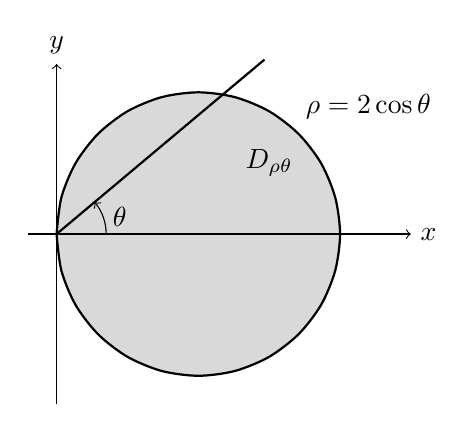
\begin{tikzpicture}[scale=1.8]
    % 极坐标网格与区域填充
    \fill[gray!30] 
        plot[domain=-90:90, smooth] (\x:{2*cos(\x)}) -- cycle;
    
    % 画出圆 \rho=2\cos\theta
    \draw[thick]
        plot[domain=-90:90, smooth] (\x:{2*cos(\x)});
    
    % 坐标轴
    \draw[->] (-0.2,0) -- (2.5,0) node[right] {$x$};
    \draw[->] (0,-1.2) -- (0,1.2) node[above] {$y$};
    
    % 一条示例射线
    \draw[thick] (0,0) -- (40:{2.5*cos(40)});
    \draw[->] (0.35,0) arc (0:40:0.35) node[midway, right] {$\theta$};
    
    % 标注
    \node at (1.5,0.5) {$D_{\rho\theta}$};
    \node at (2.2,0.9) {$\rho=2\cos\theta$};

\end{tikzpicture}
\end{center}

    
    于是三重积分化为：
    \[
    \iiint_{\Omega} (x^2+y^2)\,dV
    = \iint_{D_{\rho\theta}}\left(\int_{0}^{4} \rho^2 \, dz\right) \, \rho d\rho d\theta
    = \int_{-\frac{\pi}{2}}^{\frac{\pi}{2}} d\theta \int_{0}^{2\cos\theta} d\rho \int_{0}^{4} \rho^3 \, dz
    \]

    先对 \(z\) 积分，被积函数 \(\rho^3\) 与 \(z\) 无关，所以：
    \[
    \int_{0}^{4} \rho^3 \, dz = 4\rho^3
    \]

    再对 \(\rho\) 积分：
    \[
    \int_{0}^{2\cos\theta} 4\rho^3\,d\rho = 4\left[ \frac{\rho^4}{4} \right]_{0}^{2\cos\theta} = (2\cos\theta)^4 = 16\cos^4\theta
    \]

    最后对 \(\theta\) 积分：
    \[
    \int_{-\frac{\pi}{2}}^{\frac{\pi}{2}} 16\cos^4\theta\,d\theta
    = 32 \int_{0}^{\frac{\pi}{2}} \cos^4\theta\,d\theta
    = 32 \cdot \frac{3}{4}\cdot\frac{1}{2}\cdot\frac{\pi}{2} = 6\pi
    \]

    所以 \(\iiint_{\Omega} (x^2+y^2)\,dV = 6\pi\)。
\end{myexample}

\begin{myexample}
    计算三重积分 \(\iiint_{\Omega} z\sqrt{x^2+y^2}\,dV\)，其中 \(\Omega\) 是由圆锥面 \(z=\sqrt{x^2+y^2}\) 与平面 \(z=1\) 围成的区域。

    这个区域是一个圆锥体，顶点在原点，底面是 \(z=1\) 平面上的圆 \(x^2+y^2\le 1\)。令 \(x=\rho\cos\theta\)，\(y=\rho\sin\theta\)，\(z=z\)，则被积函数化为 \(z\cdot \rho\)，体积微元是 \(\rho\,d\rho\,d\theta\,dz\)。

    \begin{center}
    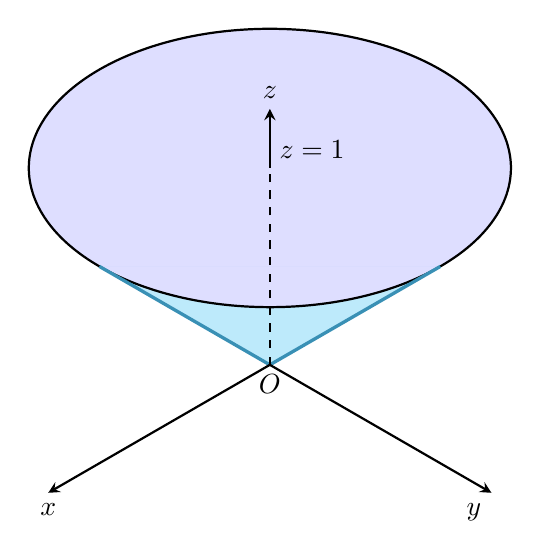
\begin{tikzpicture}[
        scale=2.5,
        line join=round,
        % 视角调整：使顶点在下，底面在上
        x={(-0.866cm,-0.5cm)},
        y={(0.866cm,-0.5cm)},
        z={(0cm,1cm)},
    ]
    
    % 圆锥参数
    \def\R{1}    % 底面半径
    \def\H{1}    % 高度
    
    % 顶点与底面圆心
    \coordinate (V) at (0,0,0);
    \coordinate (Otop) at (0,0,\H);
    
    
    \fill[cyan!40, opacity=0.65, even odd rule]
        (V) -- ({\R*cos(0)}, {\R*sin(0)}, \H) -- ({\R*cos(90)}, {\R*sin(90)}, \H) -- cycle
        % 弓形：从 A 沿弧到 B，再 -- cycle 闭合（弦 BA）
        plot[domain=0:90, samples=120, variable=\t, smooth]
            ({\R*cos(\t)}, {\R*sin(\t)}, \H)
        -- cycle;
    
    % ---- 顶面（半透明填充） ----
    \fill[blue!20, opacity=0.65]
        plot[domain=0:360, samples=120, smooth]
        ({\R*cos(\x)}, {\R*sin(\x)}, \H) -- cycle;
    
    % ---- 底面圆的轮廓线 ----
    \draw[thick]
        plot[domain=0:360, samples=120, smooth]
        ({\R*cos(\x)}, {\R*sin(\x)}, \H);
    
    
    \draw[very thick, cyan!70!black] (V) -- ({\R*cos(0)}, {\R*sin(0)}, \H);
    
    \draw[very thick, cyan!70!black] (V) -- ({\R*cos(90)}, {\R*sin(90)}, \H);
    
    
    % ---- 坐标轴（从顶点向外延伸） ----
    \draw[-stealth, thick] (V) -- (1.3,0,0) node[below] {$x$};
    \draw[-stealth, thick] (V) -- (0,1.3,0) node[below left] {$y$};
    \draw[-stealth, thick] (0,0,1) -- (0,0,1.3) node[above] {$z$};
    \draw[thick, dashed] (V) -- (0,0,1);
    
    % 标签
    \node[below] at (V) {$O$};
    \node[above right] at (0,0,\H) {$z=1$};
    
    \end{tikzpicture}
    \quad
    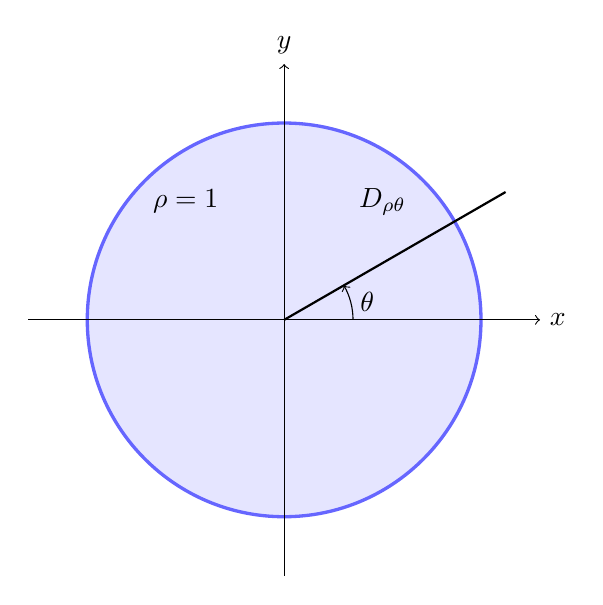
\begin{tikzpicture}[
    scale=2.5,
]
  % 填充圆盘并画出边界
  \filldraw[fill=blue!10, draw=blue!60, very thick] (0,0) circle (1);

  \draw[->] (-1.3,0) -- (1.3,0) node[right] {$x$};
  \draw[->] (0,-1.3) -- (0,1.3) node[above] {$y$}; 

  % 说明文字
  \node at (0.5,0.6) {$D_{\rho\theta}$};

  \draw[thick] (0,0) -- (30:{1.5*cos(30)});

  \draw[->] (0.35,0) arc (0:30:0.35) node[midway, right] {$\theta$};

  \node at (-0.5,0.6) {$\rho=1$};

\end{tikzpicture}
\end{center}

    接下来用“画图穿线法”确定积分限。先看 \(z\) 方向。直线从圆锥面 \(z=\rho\) 穿入，从顶面 \(z=1\) 穿出。所以 \(z\) 的积分下限是 \(\rho\)，上限是 \(1\)。
    
    再把\(\Omega\)投影到\(xOy\) 平面，得到 \(D_{\rho\theta}\)。投影区域是圆 \(\rho\le 1\)，所以 \(\theta\) 从 \(0\) 扫到 \(2\pi\)，对每一个 \(\theta\)，射线从 \(\rho=0\) 穿入，从 \(\rho=1\) 穿出。

    于是：
    \[
    \iiint_{\Omega} z\sqrt{x^2+y^2}\,dV
    =\iint_{D_{\rho\theta}} \left(\int_{\rho}^{1} (z\cdot \rho) \, dz\right) \, \rho d\rho d\theta
    = \int_{0}^{2\pi} d\theta \int_{0}^{1} \rho^2\,d\rho \int_{\rho}^{1} z \, dz
    \]

    先对 \(z\) 积分：
    \[
    \int_{\rho}^{1} z\,dz = \left[ \frac{z^2}{2} \right]_{\rho}^{1} = \frac{1}{2} - \frac{\rho^2}{2} = \frac{1-\rho^2}{2}
    \]

    再对 \(\rho\) 积分：
    \[
    \int_{0}^{1} \rho^2 \cdot \frac{1-\rho^2}{2} \, d\rho
    = \frac{1}{2} \int_{0}^{1} (\rho^2 - \rho^4) \, d\rho
    = \frac{1}{2} \left[ \frac{\rho^3}{3} - \frac{\rho^5}{5} \right]_{0}^{1}
    = \frac{1}{2} \left( \frac{1}{3} - \frac{1}{5} \right)
    = \frac{1}{2} \cdot \frac{2}{15} = \frac{1}{15}
    \]

    最后对 \(\theta\) 积分，被积函数已经是常数：
    \[
    \int_{0}^{2\pi} \frac{1}{15}\,d\theta = \frac{1}{15} \cdot 2\pi = \frac{2\pi}{15}
    \]

    所以 \(\iiint_{\Omega} z\sqrt{x^2+y^2}\,dV = \frac{2\pi}{15}\)。
\end{myexample}

总结一下，用柱面坐标计算三重积分的思路和直角坐标下的投影法一脉相承。当区域在 \(xOy\) 平面上的投影是圆、扇形或圆环，且被积函数出现 \(x^2+y^2\) 时，柱面坐标通常是最好的选择。要注意的就是体积微元的 \(\textcolor{red}{\rho}\) 绝对不能漏掉，还有“画图穿线法”判断上下限时要分别对 \(z\)、\(\theta\)、\(\rho\)依次操作，看清楚穿入和穿出的边界各是什么。

\subsection{三重积分的球面坐标形式}

当积分区域是球体、球壳或者球体的一部分，又或者被积函数里出现了 \(x^2+y^2+z^2\) 这类项，用柱面坐标有时还是会比较麻烦。这时就可以搬出球面坐标，它是专门对付球形区域的有力工具。

球面坐标用三个数来确定空间中一点的位置，分别是向径 \(r\)，方位角 \(\theta\)，以及极角 \(\varphi\)。在球面坐标里，通常取\(0\le r<+\infty\)，\(0\le|\varphi|\le\pi\)，\(0\le|\theta|\le 2\pi\)。


\begin{center}
\begin{tikzpicture}[
    scale=1.5,
    x={(1cm,0cm)},
    y={(-0.4cm,-0.35cm)},
    z={(0cm,1cm)},
    line join=round,
    line cap=round
]
    % 坐标轴
    \draw[->] (-0.2,0,0) -- (3.2,0,0) node[below] {$x$};
    \draw[->] (0,-0.2,0) -- (0,2.8,0) node[right] {$y$};
    \draw[->] (0,0,0) -- (0,0,2.8) node[left] {$z$};
    \node[below left] at (0,0,0) {$O$};

    % 定义点 P 的坐标
    \def\rr{3.2}
    \def\phii{53}
    \def\thh{45}

    % 计算点 P 的直角坐标
    \pgfmathsetmacro\xx{\rr*sin(\phii)*cos(\thh)}
    \pgfmathsetmacro\yy{\rr*sin(\phii)*sin(\thh)}
    \pgfmathsetmacro\zz{\rr*cos(\phii)}

    % 点 P
    \coordinate (P) at (\xx,\yy,\zz);
    \fill (P) circle (1.2pt) node[above right] {$M(r,\varphi,\theta)$};

    % 投影点 P' 在 xOy 平面上
    \coordinate (Pxy) at (\xx,\yy,0);
    \fill (Pxy) circle (1.2pt) node[below right] {$M'(r,\varphi,0)$};

    % 连接
    \draw[dashed] (P) -- (Pxy);
    \draw[dashed] (0,0,0) -- (Pxy);

    % 标出 r
    \draw[thick] (0,0,0) -- (P);
    \node[above] at (2*\xx/3,2*\yy/3,2*\zz/3) {$r$};

    % 标出 phi 角（在 z--P 平面内）
    \draw[->] (0,0,0.4) arc (90-\phii:90:-0.4);
    \node[right] at (0.1,0,0.6) {$\varphi$};

    % 标出 theta 角
    \draw[->] (0.6,0,0) arc (0:\thh:0.6);
    \node[right] at (0.6,0.4,0) {$\theta$};

\end{tikzpicture}
\end{center}

点 \(M(x,y,z)\) 的球面坐标与直角坐标之间的关系是\(x = r\sin\varphi\cos\theta\)，\(y = r\sin\varphi\sin\theta\)，\(z = r\cos\varphi\)。与柱面坐标的关系是\(r = \sqrt{\rho^2+z^2}\)，\(\varphi = \arctan(\frac{\rho}{z})\)，\(\theta = \theta\)。反过来，如果已知球面坐标，令\(\rho=r\sin\varphi\)，\(z=r\cos\varphi\)，\(\theta=\theta\)，就得到柱面坐标。

有了坐标变换，下一步就要弄清楚球面坐标下的体积微元是什么。和二重积分极坐标、三重积分柱面坐标的思路如出一辙，我们把 \(r,\varphi,\theta\) 各自取一个微小的增量 \(\Delta r,\Delta\varphi,\Delta\theta\)，这一小块区域近似是一个弯曲的“长方体”。在 \(r\) 方向上的边长是 \(\Delta r\)，在 \(\varphi\) 方向上的“弧长”是 \(r\,\Delta\varphi\)，在 \(\theta\) 方向上的“弧长”是 \(r\sin\varphi\,\Delta\theta\)。当这些增量都趋向于零时，也就是取微分，那么\(\Delta r\)就是\(dr\)，\(r\,\Delta\varphi\)就是\(r\,d\varphi\)，\(r\sin\varphi\,\Delta\theta\)就是\(r\sin\varphi\,d\theta\)，这时候体积微元就是这三者的乘积，所以：
\[
dV = dr \cdot r\,d\varphi \cdot r\sin\varphi\,d\theta = r^2\sin\varphi\,dr\,d\varphi\,d\theta
\]

\begin{center}
\begin{tikzpicture}[
    scale=2,
    x={(1cm,0cm)},
    y={(-0.4cm,-0.35cm)},
    z={(0cm,1cm)},
    line join=round,
    line cap=round
]
    % 坐标轴
    \draw[->] (-0.2,0,0) -- (2.4,0,0) node[below] {$x$};
    \draw[->] (0,-0.2,0) -- (0,1.8,0) node[right] {$y$};
    \draw[->] (0,0,0) -- (0,0,2.4) node[left] {$z$};
    \node[above left] at (0,0,0) {$O$};

    % 定义点 P 的坐标
    \def\rr{2.8}
    \def\phii{45}
    \def\thh{30}
    \def\drr{0.8}
    \def\dthh{15}
    \def\dphii{10}

    % 计算点 P 的直角坐标
    \pgfmathsetmacro\xx{\rr*sin(\phii)*cos(\thh)}
    \pgfmathsetmacro\yy{\rr*sin(\phii)*sin(\thh)}
    \pgfmathsetmacro\zz{\rr*cos(\phii)}
    \pgfmathsetmacro\RR{\rr+\drr}

    % 点
    \coordinate (A) at (\xx,\yy,\zz);
    \coordinate (B) at ({\rr*sin(\phii+\dphii)*cos(\thh)},{\rr*sin(\phii+\dphii)*sin(\thh)},{\rr*cos(\phii+\dphii)});
    \coordinate (C) at ({\rr*sin(\phii)*cos(\thh+\dthh)},{\rr*sin(\phii)*sin(\thh+\dthh)},{\rr*cos(\phii)});
    \coordinate (D) at ({\rr*sin(\phii+\dphii)*cos(\thh+\dthh)},{\rr*sin(\phii+\dphii)*sin(\thh+\dthh)},{\rr*cos(\phii+\dphii)});
    \coordinate (A1) at ({\RR*sin(\phii)*cos(\thh)},{\RR*sin(\phii)*sin(\thh)},{\RR*cos(\phii)});
    \coordinate (B1) at ({\RR*sin(\phii+\dphii)*cos(\thh)},{\RR*sin(\phii+\dphii)*sin(\thh)},{\RR*cos(\phii+\dphii)});
    \coordinate (C1) at ({\RR*sin(\phii)*cos(\thh+\dthh)},{\RR*sin(\phii)*sin(\thh+\dthh)},{\RR*cos(\phii)});
    \coordinate (D1) at ({\RR*sin(\phii+\dphii)*cos(\thh+\dthh)},{\RR*sin(\phii+\dphii)*sin(\thh+\dthh)},{\RR*cos(\phii+\dphii)});

    \fill[gray!50,opacity=0.5]
  (C) -- (C1)
  plot[domain=\thh+\dthh:\thh, samples=40]
    ({\RR*sin(\phii)*cos(\x)}, {\RR*sin(\phii)*sin(\x)}, {\RR*cos(\phii)})
  -- plot[domain=\phii:\phii+\dphii, samples=40]
    ({\RR*sin(\x)*cos(\thh)}, {\RR*sin(\x)*sin(\thh)}, {\RR*cos(\x)})
  -- (B)
  -- plot[domain=\thh:\thh+\dthh, samples=40]
    ({\rr*sin(\phii+\dphii)*cos(\x)}, {\rr*sin(\phii+\dphii)*sin(\x)}, {\rr*cos(\phii+\dphii)})
  -- plot[domain=\phii+\dphii:\phii, samples=40]
    ({\rr*sin(\x)*cos(\thh+\dthh)}, {\rr*sin(\x)*sin(\thh+\dthh)}, {\rr*cos(\x)})
  -- cycle;


    % 投影点 P' 在 xOy 平面上
    \coordinate (Axy) at (\xx,\yy,0);
    \coordinate (D1xy) at ({\RR*sin(\phii+\dphii)*cos(\thh+\dthh)},{\RR*sin(\phii+\dphii)*sin(\thh+\dthh)},0);

    % 连接
    \draw[dashed] (A) -- (Axy);
    \draw[dashed] (0,0,0) -- (Axy);

    \draw[dashed] (D1) -- (D1xy);
    \draw[dashed] (0,0,0) -- (D1xy);

    % 标出 r
    \draw[dashed] (0,0,0) -- (A);
    \draw[dashed] (0,0,0) -- (B);
    \draw[thick,dashed] (A) -- (A1);
    \draw[thick] (B) -- (B1);
    \draw[thick] (C) -- (C1);
    \draw[thick] (D) -- (D1);

  \draw[thick,dashed] plot[domain=\phii:\phii+\dphii, samples=80]
  ({\rr*sin(\x)*cos(\thh)}, {\rr*sin(\x)*sin(\thh)}, {\rr*cos(\x)});

  \draw[thick,dashed] plot[domain=\thh:\thh+\dthh, samples=80]
  ({\rr*sin(\phii)*cos(\x)}, {\rr*sin(\phii)*sin(\x)}, {\rr*cos(\phii)});

  \draw[thick] plot[domain=\phii:\phii+\dphii, samples=80]
  ({\rr*sin(\x)*cos(\thh+\dthh)}, {\rr*sin(\x)*sin(\thh+\dthh)}, {\rr*cos(\x)});

\draw[thick] plot[domain=\thh:\thh+\dthh, samples=80]
  ({\rr*sin(\phii+\dphii)*cos(\x)}, {\rr*sin(\phii+\dphii)*sin(\x)}, {\rr*cos(\phii+\dphii)});

  % ---------- 外层弧线 ----------
% 经线弧：A1 -> B1 (等 θ = θ₀)
\draw[thick] plot[domain=\phii:\phii+\dphii, samples=80]
  ({\RR*sin(\x)*cos(\thh)}, {\RR*sin(\x)*sin(\thh)}, {\RR*cos(\x)});

% 纬线弧：A1 -> C1 (等 φ = φ₀)
\draw[thick] plot[domain=\thh:\thh+\dthh, samples=80]
  ({\RR*sin(\phii)*cos(\x)}, {\RR*sin(\phii)*sin(\x)}, {\RR*cos(\phii)});

% 经线弧：C1 -> D1 (等 θ = θ₀ + Δθ)
\draw[thick] plot[domain=\phii:\phii+\dphii, samples=80]
  ({\RR*sin(\x)*cos(\thh+\dthh)}, {\RR*sin(\x)*sin(\thh+\dthh)}, {\RR*cos(\x)});

% 纬线弧：B1 -> D1 (等 φ = φ₀ + Δφ)
\draw[thick] plot[domain=\thh:\thh+\dthh, samples=80]
  ({\RR*sin(\phii+\dphii)*cos(\x)}, {\RR*sin(\phii+\dphii)*sin(\x)}, {\RR*cos(\phii+\dphii)});

  \draw[->] ({0.8*cos(\thh)},{0.8*sin(\thh)},0) arc(\thh:(\thh+\dthh):0.8) node[midway,below right] {$d\theta$};

  \draw[->] 
  plot[domain=\phii:\phii+\dphii, samples=80]
    ({0.8*sin(\x)*cos(\thh)}, 
     {0.8*sin(\x)*sin(\thh)}, 
     {0.8*cos(\x)})
  node[below right] {$d\varphi$};

\pgfmathsetmacro{\thetaMid}{\thh + 0.5*\dthh}
\pgfmathsetmacro{\xMid}{\rr*sin(\phii)*cos(\thetaMid)}
\pgfmathsetmacro{\yMid}{\rr*sin(\phii)*sin(\thetaMid)}
\pgfmathsetmacro{\zMid}{\rr*cos(\phii)}

% 画引线（从弧中点向外偏移 0.6cm 的向量，可按视角调整）
\draw (\xMid, \yMid, \zMid)
  -- ++(-0.5, -1.5, 0) % ← 这里控制引线方向和长度
  node[above] {$r\sin\varphi\,d\theta$};

\pgfmathsetmacro{\phiMid}{\phii + 0.5*\dphii}
\pgfmathsetmacro{\xMidCD}{\rr*sin(\phiMid)*cos(\thh+\dthh)}
\pgfmathsetmacro{\yMidCD}{\rr*sin(\phiMid)*sin(\thh+\dthh)}
\pgfmathsetmacro{\zMidCD}{\rr*cos(\phiMid)}

\draw (\xMidCD, \yMidCD, \zMidCD)
  -- ++(-0.8, -0.8, 0)               % 偏移量可调
  node[above] {$r\,d\varphi$};


\draw ($(D)!0.5!(D1)$)
  -- ++(0.4, 1.2, 0)
  node[below] {$dr$};

\end{tikzpicture}
\end{center}


由此便得到了三重积分在球面坐标下的变换公式：

\begin{theorem}{三重积分球面坐标变换公式}{}
设函数 \(f(x,y,z)\) 在空间区域 \(\Omega\) 上可积，作球面坐标变换 \(x=r\sin\varphi\cos\theta,\;y=r\sin\varphi\sin\theta,\;z=r\cos\varphi\)，则
\[
\iiint_{\Omega} f(x,y,z)\,dxdydz
= \iiint_{\Omega} f(r\sin\varphi\cos\theta,\; r\sin\varphi\sin\theta,\; r\cos\varphi)\;
r^2\sin\varphi\,dr\,d\varphi\,d\theta
\]
\end{theorem}


要注意的是，球面坐标下的体积微元是 \(\textcolor{red}{r^2\sin\varphi}\,dr\,d\varphi\,d\theta\)，既不是 \(dr\,d\varphi\,d\theta\)，也不是 \(r\,dr\,d\varphi\,d\theta\)，而是\(\textcolor{red}{r^2\sin\varphi}\,dr\,d\varphi\,d\theta\)。

在积分次序上，球面坐标和柱面坐标一样，通常采用“先一后二”的思路。对大多数区域，我们是先固定 \(\varphi\) 和 \(\theta\)，从原点引出一条射线穿过区域，确定 \(r\) 的上下限，然后再对 \(\varphi,\theta\) 在某个平面区域上做二重积分。

用“画图穿线法”操作就是固定住 \(\varphi\) 和 \(\theta\)，然后从原点出发引一条射线，这条射线穿进区域的那一点就是积分下限 \(r=r_1(\varphi,\theta)\)，穿出区域的那一点就是积分上限 \(r=r_2(\varphi,\theta)\)，再让 \((\varphi,\theta)\) 在某个参数区域 \(\Delta\) 上变化，把所有这些射线上的累积量加起来，结果就是三重积分的值。所以我们有：
\begin{theorem}{球面坐标下的三重积分}{}
若空间闭区域 \(\Omega\) 可表示为
\[
\Omega = \{(r\sin\varphi\cos\theta,\; r\sin\varphi\sin\theta,\; r\cos\varphi) \mid
(\varphi,\theta)\in\Delta,\; r_1(\varphi,\theta)\le r\le r_2(\varphi,\theta)\}
\]
则
\[
\iiint_{\Omega} f(x,y,z)\,dxdydz
= \iiint_{\Omega} F(r,\varphi,\theta)\,r^2\sin\varphi\,dr\,d\varphi\,d\theta
\]
其中\(F(r,\varphi,\theta)=f(r\sin\varphi\cos\theta,\; r\sin\varphi\sin\theta,\; r\cos\varphi)\)。
\end{theorem}

至于 \(\varphi\) 和 \(\theta\) 的范围，需要根据积分区域的具体形状来确定。

\begin{myexample}
计算三重积分 \(\iiint_{\Omega} (x^2+y^2+z^2)\,dV\)，其中 \(\Omega\) 是由球面 \(x^2+y^2+z^2=R^2\) 围成的球体。

被积函数里出现了 \(x^2+y^2+z^2\)，整个区域又是一个标准的球体，这正是球面坐标大显身手的时候。作球面坐标变换，令 \(x=r\sin\varphi\cos\theta,\; y=r\sin\varphi\sin\theta,\; z=r\cos\varphi\)，则被积函数化为 \(r^2\)，体积微元是 \(r^2\sin\varphi\,dr\,d\varphi\,d\theta\)，区域 \(\Omega\) 就是 \(0\le r\le R\)，\(0\le\varphi\le\pi\)，\(0\le\theta\le 2\pi\)。

\begin{center}
    \begin{tikzpicture}
      \tdplotsetmaincoords{56}{135}
      
      \begin{scope}[tdplot_main_coords, scale=1.5]
        \draw[->, thick] (0,0,0) -- (2.5,0,0) node[anchor=north east] {$x$};
        \draw[->, thick] (0,0,0) -- (0,2.5,0) node[anchor=north west] {$y$};
        \draw[->, thick] (0,0,0) -- (0,0,2.5) node[anchor=south]      {$z$};
        \shade[ball color=blue!25] (0,0,0) circle (1.5cm);
      \end{scope}
    \end{tikzpicture}
\end{center}

所以：
\[
\iiint_{\Omega} (x^2+y^2+z^2)\,dV
= \iiint_{\Omega} r^2\cdot r^2\sin\varphi\,dr\,d\varphi\,d\theta
= \int_{0}^{2\pi} d\theta \int_{0}^{\pi}\sin\varphi \,d\varphi \int_{0}^{R} r^4\,dr
\]

先对 \(r\) 积分：
\[
\int_{0}^{R} r^4\,dr = \left[ \frac{r^5}{5} \right]_{0}^{R} = \frac{R^5}{5}
\]

再对 \(\varphi\) 积分：
\[
\int_{0}^{\pi} \frac{R^5}{5}\sin\varphi\,d\varphi = \frac{R^5}{5}\bigl[-\cos\varphi\bigr]_{0}^{\pi} = \frac{2R^5}{5}
\]

最后对 \(\theta\) 积分：
\[
\int_{0}^{2\pi}\frac{2R^5}{5}\,d\theta =\frac{2R^5}{5}\cdot 2\pi=\frac{4\pi R^5}{5}
\]

所以 \(\iiint_{\Omega} (x^2+y^2+z^2)\,dV = \dfrac{4\pi R^5}{5}\)。
\end{myexample}

\begin{myexample}
计算三重积分 \(\iiint_{\Omega} z\,dV\)，其中 \(\Omega\) 是由上半球面 \(x^2+y^2+z^2=1,\; z\ge 0\) 与圆锥面 \(z=\sqrt{x^2+y^2}\) 所围成的位于锥面下方的区域。

这个区域看起来有点复杂，但用球面坐标描述就非常自然。令 \(x=r\sin\varphi\cos\theta,\; y=r\sin\varphi\sin\theta,\; z=r\cos\varphi\)，则被积函数化为 \(r\cos\varphi\)，体积微元是 \(r^2\sin\varphi\,dr\,d\varphi\,d\theta\)。

先看看区域的边界。球面是 \(r=1\)。圆锥面 \(z=\sqrt{x^2+y^2}\) 化为球面坐标就是 \(r\cos\varphi = r\sin\varphi\)，即 \(\tan\varphi=1\)，也就是 \(\varphi=\frac{\pi}{4}\)。区域在锥面下方，即 \(z\le\sqrt{x^2+y^2}\)，对应 \(\cos\varphi\le\sin\varphi\)，所以 \(\varphi\) 从 \(\frac{\pi}{4}\) 到 \(\frac{\pi}{2}\)，也就是\(\varphi\in [\frac{\pi}{4},\frac{\pi}{2}]\)。\(\theta\) 可以绕区域一圈，所以 \(\theta\in [0,2\pi]\)。对于每一个固定的 \((\varphi,\theta)\)，射线从原点出发，先进入区域，穿进区域时是原点 \(r=0\)，穿出来碰到球面就是 \(r=1\)。所以 \(r\) 的范围是 \(0\le r\le 1\)。

\begin{center}
\begin{tikzpicture}[scale=2.5]
  \tdplotsetmaincoords{70}{120}
\begin{scope}[tdplot_main_coords]
  
  % ========== 基本常量 ==========
  \def\R{1}                     % 球半径
  \pgfmathsetmacro{\h}{1/sqrt(2)} % 交线高度
  \pgfmathsetmacro{\r}{\h}       % 交线半径

  
  
  % ========== 根据视角定义可见角度范围 ==========
  % 可见弧从 phi_start 到 phi_end（度）
  \def\phistart{-60}
  \def\phiend{120}
  % 不可见弧的结束角（360 + phistart 的等价正角度）
  \def\phihideend{300}  % 即 -40° + 360°
  
  % ========== 1. 不可见部分（虚线） ==========
  % 赤道圆（z=0）的不可见弧
  \draw[cyan, densely dashed, thick]
    ({\R*cos(\phiend)}, {\R*sin(\phiend)}, 0)
    arc[start angle=\phiend, end angle=\phihideend, radius=\R];
  
  \fill[red!80, opacity=0.72]
  plot[domain=0:360, smooth, variable=\t]
    ({\r*cos(\t)}, {\r*sin(\t)}, \h) -- cycle;

  
  % ========== 2. Ω 区域的可见表面（透明填充） ==========
  % 锥面可见部分（原点 → 左母线 → 交线可见弧 → 右母线 → 原点）
  \def\phicontourA{98.66}
  \def\phicontourB{-38.66}


  \fill[red!80, opacity=0.72]
    (0,0,0) --
    ({\r*cos(\phicontourA)}, {\r*sin(\phicontourA)}, \h) --
    plot[domain=\phicontourA:\phicontourB, smooth, variable=\phi]
      ({\r*cos(\phi)}, {\r*sin(\phi)}, \h) --
    cycle;

    
% 画两条轮廓母线（实线）
\draw[red!80, thick, dashed]
  ({\r*cos(\phicontourA)}, {\r*sin(\phicontourA)}, \h) -- (0,0,0)
  ({\r*cos(\phicontourB)}, {\r*sin(\phicontourB)}, \h) -- (0,0,0);
  
  % 球面可见部分（交线可见弧 + 赤道可见弧围成的区域）

  \pgfmathsetmacro{\latTop}{asin(\h)}   % 顶部纬度 (弧度)
  \pgfmathsetmacro{\latBottom}{0}       % 底部纬度

% 侧面填充
\fill[cyan, opacity=0.2]
    % 1. 底部纬线弧 (z=0, 半径 R=1)
    ({\R*cos(\phistart)}, {\R*sin(\phistart)}, 0)
    arc[start angle=\phistart, end angle=\phiend, radius=\R]
    
    % 2. 右侧经线弧：经度固定为 \phiend，纬度从 \latBottom 到 \latTop
    %    参数方程: (cosγ·cosφ, cosγ·sinφ, sinγ)
    -- plot[domain=\latBottom:\latTop, variable=\gamma]
        ({cos(\gamma)*cos(\phiend)}, {cos(\gamma)*sin(\phiend)}, {sin(\gamma)})
    
    % 3. 顶部纬线弧 (z=h, 半径 r, 反向从 \phiend 到 \phistart)
    arc[start angle=\phiend, end angle=\phistart, radius=\r]
    
    % 4. 左侧经线弧：经度 \phistart，纬度从 \latTop 回到 \latBottom
    -- plot[domain=\latTop:\latBottom, variable=\gamma]
        ({cos(\gamma)*cos(\phistart)}, {cos(\gamma)*sin(\phistart)}, {sin(\gamma)})
    -- cycle;
  
    % 右侧经线轮廓 (φ = φend)
\draw[cyan, thick]
  plot[domain=0:\latTop, variable=\gamma]
    ({cos(\gamma)*cos(\phiend)}, {cos(\gamma)*sin(\phiend)}, {sin(\gamma)});
% 左侧经线轮廓 (φ = φstart)
\draw[cyan, thick]
  plot[domain=0:\latTop, variable=\gamma]
    ({cos(\gamma)*cos(\phistart)}, {cos(\gamma)*sin(\phistart)}, {sin(\gamma)});
  % ========== 3. 可见轮廓与结构线（实线） ==========
  % 赤道圆可见弧
  \draw[cyan, thick]
    ({\R*cos(\phistart)}, {\R*sin(\phistart)}, 0)
    arc[start angle=\phistart, end angle=\phiend, radius=\R];
  
  % 交线圆可见弧
  \draw[red!80, thick] 
    plot[domain=0:360, smooth, samples=120, variable=\t] 
    ({\r*cos(\t)}, {\r*sin(\t)}, \h) -- cycle;
  
    \draw[dashed, thick] (0,0,0) -- (1,0,0);
  \draw[-stealth, thick] (1,0,0) -- (1.3,0,0) node[anchor=north east]{$x$};
  \draw[dashed, thick] (0,0,0) -- (0,1,0);
  \draw[-stealth, thick] (0,1,0) -- (0,1.3,0) node[anchor=north west]{$y$};
  \draw[dashed, thick] (0,0,0) -- (0,0,{1/sqrt(2)});
  \draw[-stealth, thick] (0,0,{1/sqrt(2)}) -- (0,0,1.3) node[anchor=south]{$z$};



  % ========== 4. 标签 ==========
  \node at (0.9, 0.15, 0.5) {\(\Omega\)};
  
\end{scope}
\end{tikzpicture}
\end{center}

于是：
\[
\iiint_{\Omega} z\,dV
= \iiint_{\Omega} r\cos\varphi\cdot r^2\sin\varphi\,dr\,d\varphi\,d\theta
= \int_{0}^{2\pi} d\theta \int_{\frac{\pi}{4}}^{\frac{\pi}{2}} \sin\varphi\,d\varphi \int_{0}^{1} r^3\cos\varphi\,dr
\]

先对 \(r\) 积分，\(\cos\varphi\) 与 \(r\) 无关：
\[
\int_{0}^{1} r^3\cos\varphi\,dr = \cos\varphi\left[ \frac{r^4}{4} \right]_{0}^{1} = \frac{\cos\varphi}{4}
\]

再对 \(\varphi\) 积分：
\[
\int_{\frac{\pi}{4}}^{\frac{\pi}{2}} \frac{\cos\varphi}{4} \sin\varphi\,d\varphi
= \frac{1}{4} \int_{\frac{\pi}{4}}^{\frac{\pi}{2}} \sin\varphi\cos\varphi\,d\varphi
= \frac{1}{8} \int_{\frac{\pi}{4}}^{\frac{\pi}{2}} \sin 2\varphi\,d\varphi
= \frac{1}{8} \left[ -\frac{\cos 2\varphi}{2} \right]_{\frac{\pi}{4}}^{\frac{\pi}{2}}
= \frac{1}{16}
\]

最后对 \(\theta\) 积分：
\[
\int_{0}^{2\pi} \frac{1}{16}\,d\theta = \frac{1}{16} \cdot 2\pi = \frac{\pi}{8}
\]

所以 \(\iiint_{\Omega} z\,dV = \dfrac{\pi}{8}\)。
\end{myexample}

总结一下，球面坐标主要是为球体和球壳一类问题准备的。当被积函数含有 \(x^2+y^2+z^2\)，或者区域边界是球面、锥面时，球面坐标往往比柱面坐标还要方便。使用时要牢记体积微元是 \(\textcolor{red}{r^2\sin\varphi}\,dr\,d\varphi\,d\theta\)。确定积分限时，用“画图穿线法”从原点引射线，穿入和穿出的位置分别是 \(r\) 的上下限，再根据区域在 \((\varphi,\theta)\) 上的投影确定角度范围，最后按 \(r\)、\(\varphi\)、\(\theta\) 的顺序化为累次积分即可。

至此，从二重积分到三重积分的几种常用坐标计算法就都介绍完了。不管面对什么形式的积分，只要抓住“分割、近似、求和、取极限”的核心思想，再结合区域的特点选择合适的坐标系，二重积分和三重积分就都不是难事。